%! TEX root = main.tex
\documentclass[12pt, a4paper]{article}

\usepackage{graphicx} % Required for inserting images
\usepackage[utf8]{inputenc}
\usepackage[english, russian]{babel}
\usepackage{times}
\usepackage{fontspec} 
\usepackage{titlesec}
\usepackage{amsmath}
\usepackage[normalem]{ulem}
\usepackage[htt]{hyphenat}
\usepackage{amssymb}
\usepackage{mathtools}
\usepackage{wrapfig}
\usepackage{tabularx}
\usepackage{svg}
\usepackage{subcaption}
\usepackage{pdfpages}
\renewcommand{\thesubfigure}{\asbuk{subfigure}} % а, б, в...
\usepackage[normalem]{ulem}
\numberwithin{equation}{section}
\defaultfontfeatures{Ligatures={TeX},Renderer=Basic} 
\usepackage{appendix}
\setmainfont[Ligatures={TeX,Historic}]{Times New Roman}

% \usepackage{polyglossia}
% \setmainlanguage[Script=Cyrillic]{russian}

\usepackage{biblatex}
\addbibresource{sources.bib}

\usepackage{indentfirst}
\setlength\parindent{12.5mm}

\usepackage{geometry}
% \geometry{
%     a4paper,
%     left=30mm,
%     right=10mm,
%     top=20mm,
%     bottom=20mm
% }
\geometry{
  a4paper,
  top=2cm,
  bottom=2cm,
  left=2.5cm,
  right=1cm
} %, heightrounded, showframe

\usepackage{array,supertabular,hhline,enumitem,hyperref}
\usepackage{listings}
\usepackage{xcolor}
\usepackage{longfbox,fancyhdr}
\definecolor{codegreen}{rgb}{0,0.6,0}
\definecolor{codegray}{rgb}{0.5,0.5,0.5}
\definecolor{codepurple}{rgb}{0.58,0,0.82}

\lstset{
    backgroundcolor=\color{white},
    commentstyle=\color{codegreen},
    keywordstyle=\color{magenta},
    numberstyle=\tiny\color{codegray},
    stringstyle=\color{codepurple},
    basicstyle=\ttfamily\footnotesize,
    breakatwhitespace=false,
    breaklines=true,
    captionpos=t,
    keepspaces=true,
    numbers=left,
    numbersep=5pt,
    showspaces=false,
    showstringspaces=false,
    showtabs=false,
    tabsize=2,
    frame=single,
}

\lstset{
    rangeprefix=\#\ SECTION\ ,
    % rangebeginprefix=\#\ SECTION,
    % rangeendprefix=#\ SECTION,
    rangebeginsuffix=\ BEGIN,
    rangeendsuffix=\ END,
    includerangemarker=false
}

\newcommand\listingsection[2]{
  \lstinputlisting[
    language=python,
    linerange=#2-#2
  ]{#1}
}

\let\stdsection\section
\renewcommand\section{\clearpage\stdsection}

\usepackage{setspace}
\onehalfspacing


%%% Основные сведения %%%
\newcommand{\thesisAuthorLastName}{Скоробогатов}
\newcommand{\thesisAuthorOtherNames}{Егор Викторович}
\newcommand{\thesisAuthorInitials}{Е. В.}
\newcommand{\thesisAuthor}             % Диссертация, ФИО автора
{%
    \texorpdfstring{% \texorpdfstring takes two arguments and uses the first for (La)TeX and the second for pdf
        \thesisAuthorLastName~\thesisAuthorOtherNames% так будет отображаться на титульном листе или в тексте, где будет использоваться переменная
    }{%
        \thesisAuthorLastName, \thesisAuthorOtherNames% эта запись для свойств pdf-файла. В таком виде, если pdf будет обработан программами для сбора библиографических сведений, будет правильно представлена фамилия.
    }
}
\newcommand{\thesisAuthorShort}        % Диссертация, ФИО автора инициалами
{\thesisAuthorInitials~\thesisAuthorLastName}
%\newcommand{\thesisUdk}                % Диссертация, УДК
%{\fixme{xxx.xxx}}
\newcommand{\thesisTitle}              % Диссертация, название
{Визуальная система телеоперации манипулятором с двухпальцевым захватом}
\newcommand{\thesisSpecialtyNumber}    % Диссертация, специальность, номер
{15.03.06}
\newcommand{\thesisSpecialtyTitle}     % Диссертация, специальность, название (название взято с сайта ВАК для примера)
{Мехатроника и робототехника}
\newcommand{\thesisDegree}             % Диссертация, ученая степень
{бакалавра}
\newcommand{\thesisDegreeShort}        % Диссертация, ученая степень, краткая запись
{бак.}
\newcommand{\thesisCity}               % Диссертация, город написания диссертации
{Москва}
\newcommand{\thesisYear}               % Диссертация, год написания диссертации
{\the\year}
\newcommand{\thesisOrganization}       % Диссертация, организация
{
  Федеральное Государственное Бюджетное
  Образовательное Учреждение Высшего Образования <<Национальный
  Исследовательский Университет <<МЭИ>>
}


\newcommand{\supervisorFio}              % Научный руководитель, ФИО
{Адамов Борис Игоревич}
\newcommand{\supervisorRegalia}          % Научный руководитель, регалии
{доц.}
\newcommand{\supervisorFioShort}         % Научный руководитель, ФИО
{Б. И. Адамов}
\newcommand{\supervisorRegaliaShort}     % Научный руководитель, регалии
{доц.}

\newcommand{\wideunderline}[2][2em]{%
  \underline{\makebox[\ifdim\width>#1\width\else#1\fi]{#2}}%
}


\begin{document}
\onehalfspacing

% \begin{wrapfigure}{L}{\textwidth}
%   
\includegraphics[width=0.156\textwidth]{images/mpei_logo.jpg}
% \end{wrapfigure}
\begin{center}

\textbf{МИНОБРНАУКИ РОСИИ}\\
федеральное государственное бюджетное образовательное
учреждение высшего образования
\textbf{<<Национальный исследовательский университет <<МЭИ>>}
\end{center}
\hrule 

\hfill

\textbf{Институт} \hfill \wideunderline[6em]{ЭнМИ} \par
\textbf{Кафедра} \hfill \wideunderline[6em]{РМДиПМ}\par
\begin{center}
\large\textbf{
ЗАДАНИЕ
НА ВЫПУСКНУЮ КВАЛИФИКАЦИОННУЮ РАБОТУ
(БАКАЛАВРСКУЮ РАБОТУ)
}
\end{center}

\uline{\textbf{Направление} \hfill \thesisSpecialtyNumber \
\thesisSpecialtyTitle}\par

\uline{
  \textbf{Образовательная программа} 
  Компьютерные технологии управления
  в робототехнике и мехатронике
}\par

\uline{\textbf{Форма обучения} \hfill очная}\par

\uline{\textbf{Тема:} \hfill \thesisTitle}


\uline{Студент \hfill С-12а-21 \hfill \thesisAuthorLastName \
\thesisAuthorInitials \par}

\par

\uline{
  Руководитель ВКР \hfill к.ф.-м.н. \hfill доцент \hfill \qquad \hfill Адамов Б. И.
}\par

\newpage


\section{Введение}
С развитием машинного обучения и его применения в робототехнике, выросла
нужда в записи данных для обучения моделей, управляющих роботами. Также
очень полезной практикой является запись данных в реальных и разных
условиях. Запись часто происходит через комплекты виртуальной реальности или
специализированную аппаратуру\cite{umi}. 

Очки виртуальной реальности в комплекте с джойстиками стоят дорого и не очень
удобны из-за своей тяжести. Если сделать систему для записи действий человека,
которая будет легковесной и дешевой, то можно будет записывать движения
человека в любом месте, практически при любых условиях. Чтобы сделать систему
как можно более легковесной, ее можно реализовать при помощи камер. 

В данной работе представлена система для определения трехмерного
положения кисти в пространстве с использованием двух камер. Эта система
может использоваться для записи датасетов для обучения роботов построению
траекторий, управлению мехатронными телами, а также для простого
запоминания повторяемых действий. Система включает в себя модули
калибровки камер, распознавания рук и расчета положения рук в трехмерном
пространстве, что позволяет точно определять координаты ключевых точек рук в
реальном времени. 

Я не буду фокусироваться на алгоритмах управления в своей работе. В данной
работе подразумевается, что для робота, для которого будет использоваться моя
система уже реализовано управление в декартовом пространстве. Фокус этой работы
находится на реконструкции координат руки в выбранной системе отсчета.

\section{Постановка задачи}
В своей работе я буду создавать систему для определения положения руки в
трехмерном пространстве и приведения ее к виду двухпальцевого захвата
манипулятора.
Блок-схема задачи изображена на рисунке ~\ref{fig:problem_block_scheme}. 
\begin{figure}[h!]
  \begin{center}
    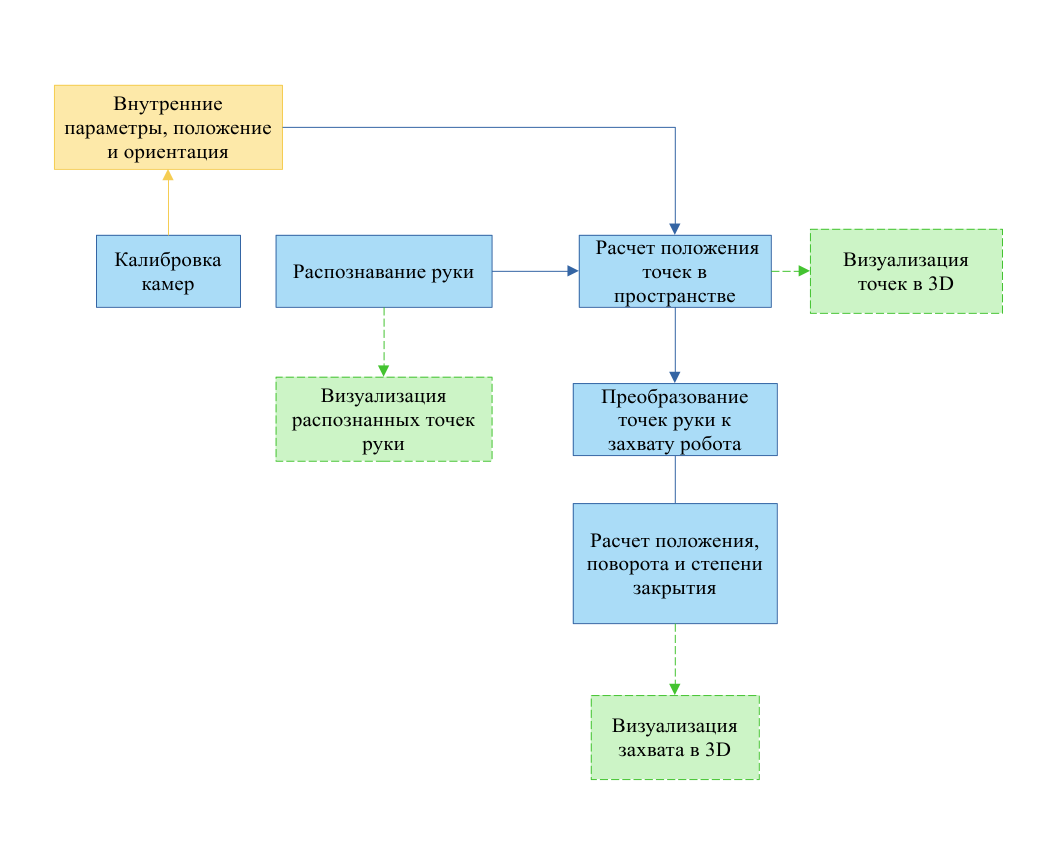
\includegraphics[width=0.95\textwidth]{images/block-schemes/problem_scheme.png}
  \end{center}
  \caption{
    Блок-схема поставленной задачи. Синим обозначены основные
    исполняемые модули, зеленым --- вспомогательные модули, а жёлтым ---
    данные.
  }
\label{fig:problem_block_scheme}
\end{figure}

\subsection{Калибровка камер}
Как далее будет сказано, у камер есть ряд параметров, которые необходимы для
корректного расчета координат в трехмерном пространстве. Некоторые из этих
параметров, такие как положение и поворот могут меняться, однако другие
параметры, о которых сказано в разеделе \ref{sec:camera_model} являются
постоянными.  Система, которую я пишу в рамках этой работы должна быть способна
найти эти параметры, то есть откалибровать камеру.
\par
Также для корректного определения положения точки в пространстве относительно
камеры, нужно знать положение камер относительно заданной точки отсчета системы
координат. То есть система также должна будет определить положение камер
относительно как либо отмеченного начала координат.

\subsection{Получение изображений и их обработка}
Часть системы, ответственная за обработку изображений должна будет выполнять следующие вещи:
\begin{itemize}
    \item принимать на вход либо устройство ввода, то есть камеру или видео,
    \item открывать это видео для захвата изображений,
    \item проводить какую-то обработку, если такая требуется,
    \item и передавать обработанное изображение дальше.
\end{itemize} 

\subsection{Распознавание руки}
Обработанное изображение должно передаваться детектору рук. Детектор рук отвечает за выполнение следующих пунктов:
\begin{itemize}
    \item нахождение ключевых точек руки, таких как шарниры между костями,
    \item обозначение их положения на изображении,
    \item передача координат и, возможно, изображений далее.
\end{itemize}   

\subsection{Расчет положения точек в пространстве}
Модуль определения положения точек должен будет:
\begin{itemize}
    \item принимать набор координат, обозначающих ключевые на изображениях с камер,
    \item расчитывать положение каждой точки относительно заданной точки отстчета,
    \item передавать эту информацию дальше.
\end{itemize}

\subsection{Преобразование точек руки к захвату робота и расчет его положения и ориентации}
Модуль преобразования трехмерной модели руки должен будет:
\begin{itemize}
    \item принимать набор координат точек в трехмерном пространстве, представляющих собой ключевые точки руки,
    \item выделять среди них характерные точки, которые нужны чтобы преобразовать руку к захвату,
    \item строить модель захвата на основе выделенных характерных точек,
    \item расчитывать положение и поворот захвата манипулятора на основе модели захвата в трехмерном пространстве.
\end{itemize}


\section{Анализ предыдущих работ}
\subsection{Телеоперация}
  Перед тем, как приступить к работе, стоит ознакомиться с телеоперацией. Я
  нашел обширную обзорную статью про телеоперацию~\cite{teleop-survey}. В этой
  статье описано что такое телеоперация, ее современные применения и способы
  реализации. Телеоперация --- управление роботом, находящимся на удалении.
  Зачастую под телеоперацией подразумевают управление, осуществляющее
  человеком. Самый простой пример телеоперции --- игрушечная радиоуправляемая
  машинка. Телеоперация нужна для самых разных вещей: 
  \begin{itemize}
    \item вмешательство человека в ситуациях, где робот не может действовать автономно,
    \item управление роботами в труднодоступных местах, например, во время хирургической или спасательой операции,
    \item запись движений человека для дальнейшего воспроизведения.
  \end{itemize}
  В своей работе я буду фокусироваться на телеоперации манипуляторами. Точнее
  на получении координат для нее. Также, была рассмотрена статья
  \cite{model-teleop}. В ней описан способ борьбы с задержкой при
  телеоперации. Суть способа в том, чтобы иметь модель системы, которая будет
  применяться для того, чтобы оператор сразу видел приблизительный результат
  своих действий.

  Когда я искал предыдущие работы про визуальную телеоперацию, я нашел две
  работы, которые по содержанию практически идентичны моей, но с небольшими
  отличиями. Первая из работ, которую я нашел называется
  AnyTeleop~\cite{anyteleop}. В своей работе авторы реализовали систему для
  детекции руки, переноса состояния кисти на захват манипулятора и планирования
  движений. Моя работа сильно похожа на эту, но я не использую нейросетевые
  методы для определения положения руки, также целевой вид захвата в моей
  работе --- двухпальцевый, в отличие от AnyTeleop. Помимо этого, я провожу
  калибровку камер, что не делается в \cite{anyteleop}. Также есть другая
  работа от J. Kofman и др.\cite{literally-me}, в которой реализованы вещи,
  идентичные тем, что будут реализованы в моей работе. Отличие этой работы от
  моей в том, что в ней реализуются методы сглаживания движения и значительная
  часть фокуса лежит на них. Я сглаживания в своей работе не касался. 
  Статью \cite{literally-me} я нашел уже после того, как большая часть задач
  была сделана, поэтому ее вклад в мою работу был минимальным.


  

\subsection{Распознавание рук}
  В начале я решил изучить то, как распознаются руки без специальных маркеров.
  Все работы, что я нашел используют нейросетевые метода для распознавания рук.
  Есть множество работ про наборы данных для обучения моделей для распознавания
  рук, например \cite{interhand}. Эта работа фокусируется на создании датасета,
  который будет содержать в себе трехмерные данные для нескольких рук
  одновременно. К сожалению, эта работа фокусируется на обучении нейронных
  сетей для одной специфичной темы, поэтому пользы не очень много. Некоторый
  интерес предоставляла \cite{dl-depth-estimation} ---  работа, в которой
  рассматривают способы оценки глубины изображения с одной камеры при помощи
  глубинного обучения. Также, я рассмотрел работу
  \cite{multiviewbootstrapping}. Эта работа фокусируется на сборе данных для
  распознавания ключевых точек руки на одном изображении. В дальнейшем, работы
  \cite{interhand, multiviewbootstrapping} могут быть полезны, если я буду
  тренировать свою модель для распознавания руки и определения ее трехмерного
  положения, но на данный момент я буду использовать уже готовые модели.


  Главное, что я нашел про распознавание рук на изображении было
  MediaPipe~\cite{mediapipe_paper} от Google. Они предоставляют API для разных
  задач, в том числе, распознавания ключевых точек руки~\cite{mediapipe_hands}
  на одном изображении. В \cite{mediapipe_hands} рассматривается распознавание
  ключевых точек для одной руки и двухмерных координат. Однако там не
  рассмытриются стереокамеры и трехмерные координат. MediaPipe много где
  используется и продвигается как вещь, способная работать на даже маломощном
  железе, поэтому для распознавания рук я решил использовать ее.
    
\subsection{Подходы к калибровке камер}
Поиски необходимой информации для калибровки много времени не заняли.
Существует библиотека OpenCV~\cite{opencv}, в котороый реализованы различные
способы калибровки, в частности --- калибровка камер с использованием досок
ChArUco~\cite{opencv_charuco}. В~\cite{opencv_charuco} авторы демонстрируют,
что такой метод позволяет уменьшить ошибку репроекции до 0.2--0.5 пикселей.

Также я наткнулся на \cite{three-stereo-principals} --- описание общих приципов
калибровки стерео камер, что актуально для моей работы. Еще интерес вызвала
\cite{camera-self-calibration} --- статься, про оценку парамеров камеры на
основе нескольких последовательных изображений с камеры.

В своей работе, я разделяю калибровку на два этапа:
\begin{enumerate}
    \item калибровка внутренних характеристик камеры,
    \item калибровка положения камер.
\end{enumerate}
На первом этапе используется доска ChArUco. Здесь калибровка проводится
аналогично с~\cite{opencv_charuco}. Во втором этапе, оценка положения камер
может проводиться при помощи разных маркеров, но принципиально калибровка
положения просто оценивает вектор поворота и смещения маркера, который был
распознан на камере, что описано не в статье, а в документации на
OpenCV~\cite{opencv_charuco_pose}. Также второй этап можно проводить независимо
для камер, однако необходимо, чтобы точка, относительно которой будет считаться
положение и поворот была одинаковой для обеих камер.

\subsection{Триангуляция ключевых точек}
Триангуляция известна очень давно и статей про нее множество, но в своей работе
я хотел бы использовать наиболее классический вариант. В
книге~\cite{multiview_cv} описаны наиболее важные концепции и алгоритмы для
компьютерного зрения с несколькими камерами, в частности описан алгоритм
триангуляции. Статья \cite{basics-of-reconstruction} рассказывает про основные
идеи конкретно для реконструкции трехмерной сцены, что будет полезно.
В~\cite{dlt_temugeb} рассказывается как реализовать и применить алгритм
триангуляции из \cite{multiview_cv}. К \cite{dlt_temugeb} я обращался чтобы
посмотреть "простое" объяснение алгоритма. Также, в \cite{multiview_cv} описан
несколько более продвинутый способ минимизации шума, нежели в
\cite{dlt_temugeb}, однако, на ранних этапах прототипирования я реализовал
более простой метод и надобности переходить к методу из \cite{multiview_cv} не
возникло.

\subsection{Преобразование руки к захвату манипулятора}
На тему распознавания жестов есть множество статей. В обзорной статье
\cite{gesture-survey} расмотрены современные методы распознавания жестов.
У \cite{mediapipe_paper} есть отдельная секция про классификацию жестов.
Однако, почти у всех статей про распознавание жестов, что я нашел есть одна
проблема --- они фокусируются на задаче классификации. Почти все статьи про
жестны рассматривают распознвавание как задчу с дискретным ответом: жест А или
жест Б. Это не подходит для моей работы, так как мне нужно знать расстояние, на
которое нужно раскрыть захват манипулятора.

В работе \cite{literally-me} переход осущетсвляется благодаря расстоянию между
кончиками указательного и большого пальцев. Это самый простой и очевидный
способ. В~\cite{gesture_control} тоже предложен эвристический метод, основанный
на расстоянии между кончиками пальцев, что близко к "простому способу",
описанному в \ref{sec:gripper_basic_method}.
\section{Выбор инструментов}
На основе списка поставленных задач и описанной теории, необходимой для их
реализации, я выбрал набор инструментов, при помощи которых я буду
реализовывать систему, описанную ранее.

Для этой работы стоял выбор между двумя языками: C++ и Python. 
C++ хорош своим быстродействием, а также обширным набором библиотек. Помимо
этого, есть ряд преимуществ, которые больше связаны с личными предпочтениями.
Однако, C++ имеет один ключевой для этой работы недостаток. По моим и не только
моим наблюдениям, реализация одного и того же программного продукта на C++
займет значительно большее время, чем реализация этого же программного продукта
на Python.

Среди преимуществ Python можно выделить простоту использования, а также высокую
читаемость кода. Как было сказано выше, программы на Python пишутся быстрее и
проще, чем на C++. Однако из недостатков Python имеет крайне малую скорость
работы, отсутствие указателей, отсутствие строгой типизации, полностью
динамическую типизацию и ряд других вещей. Так или иначе, Python гораздо лучше
подходит для прототипирования, чем C++, а в своей работе, я делаю скорее
прототип, нежели полноценный продук, я буду использовать Python.

Для работы с видео и изображениями и их обработки отлично подходит библиотека
OpenCV, доступная для C++ и Python. У меня есть опыт работы с ней, к тому же
она широко известна, хорошо задокументирована и постоянно обновляется.
Для работы с видео также можно было использовать ffmpeg\cite{ffmpeg}.
Это очень обширный инструмент с хорошей документацией, но у меня сильно больше
опыта с OpenCV, поэтому я буду использовать этот вариант.

Для калибровки камер сущетсвует хорошо задокументированные методы в
OpenCV\cite{opencv_calibration_tutorial, opencv_charuco_pose}, которые
позволяют без особых сложностей получить матрицу камеры. Также, для определения
матрицы проекции понадобится какой-то инструмент для работы с матрицами и
поворотами. Для этого я буду использовать классические бибиотеки для Python:
NumPy и SciPy. NumPy в первую очередь нужен для более быстрой и удобной работы
с массивами и матрицами так как предоставляет огромное множество полезных
методом. SciPy в своей работе я в основном использую для работы с поворотами и
их преобразованиями, так как SciPy реализует все эти методы со множеством
оптимизаций, лучше использовать их.

Для распознавания ключевых точек руки не было обширного выбора, главное, что
предлагалось в нескольких коротких статьях, что я нашел --- MediaPipe от
Google\cite{mediapipe_paper}. Это библиотека для Python и ряда других языков,
которая дает веса модели и API для взаимодействия с этой моделью для выделения
ключевых точек рук. В целом, эта библиотека имеет ряд неплохих примеров
использования и документацию. Примеры были очень полезны.
Также, чуть позже, уже после того, как был реализован модуль детекции, я нашел
альтернативу --- OpenPose. Однако применять ее времени уже нет.

Для триангуляции можно было использовать готовое решение, но я решил написать
свою версию. Так как по своей сути триангуляция является просто работой с
матрицами, то все, что для нее потребуется --- это библиотеки NumPy и SciPy.
Как ранее сказано, NumPy нужен для работы с матрицами, SciPy --- для работы с
поворотами.

Для визуализации, чтобы реализация была как можно проще и имела как можно
меньше нестандартных зависимостей, для визуализации я буду использовать
библиотеку matplotlib для Python, которая позволяет строить графики в
трехмерном пространстве. Точки я буду визуализировать через нее.

\section{Калибровка камер}
Для начала, нужно откалибровать внутренние параметры камер, которые различны
для всех камер и определяются использованной моделью камеры. Существует
множество разных моделей, однако большая часть моделей нужна для специфичных
камер, например для камеры "рыбий глаз" существует отдельная модель. Камеры
которые я использую --- Xiaovv XVV-3320S-USB --- не имеет выделяющихся
параметров, поэтому для нее можно использовать стандартную модель стенопа,
также называемую пинхол-камерой или лохкамерой.

\subsection{Модель камеры и внутренние параметры}
\label{sec:camera_model} 
В своей работе для определения параметров внутренних
параметров камеры, я использую стеноп как модель камеры. Эта модель
предстваляет камеру как совокупность двух объектов: точки в пространстве и
плоскости, расположенной на некотором удалении от этой точки. На рисунках
\ref{fig:pinhole_model} и
~\ref{fig:pinhole_geometry}, взятых из~\cite{multiview_cv} изображена данная
модель камеры.

%TODO точно ли формат подписи у рисунков такой: "Рисунок --- Название с большой буквы"
\begin{figure}[h!]
  \centering
  \includesvg[width=1\textwidth]{images/camera_model/camera_model_rus.svg}
  \caption{Модель стенопа}
~\label{fig:pinhole_model}
\end{figure}

\begin{figure}[h!]
  \centering
  \includesvg[width=0.7\textwidth]{images/camera_model/camera_model_side_rus.svg}
  \caption{Модель в проекции на плоскость YZ, f --- фокусное расстояние}
~\label{fig:pinhole_geometry}
\end{figure}

При использовании данной модели, точка $\overline{A} = (X_A, Y_A, Z_A)^T$ в
системе координат $C_{XYZ}$ проецируется на плоскость изображения по уравнению
~\eqref{eqn:pinhole_projection}, описанному в~\cite{multiview_cv}:

\begin{equation}
    \overline{A} = (X_A, Y_A, Z_A)^T \rightarrow (fX_A/Z_a, fY_A/Z_A)^T = \overline{a}.
~\label{eqn:pinhole_projection}
\end{equation}.

Уравнение \eqref{eqn:pinhole_projection} проецирует вектор из $\mathbb{R}^3$ в
пространство $\mathbb{R}^2$. Подобное преобразование можно выписать в матричной
форме через однородные преобразования, как это было сделано в книге~\cite{multiview_cv}:
\begin{equation}
    \begin{pmatrix}
        f X_A \\
        f Y_A \\
        Z_A
    \end{pmatrix} = 
    \begin{bmatrix}
        f & 0 & 0 & 0 \\
        0 & f & 0 & 0 \\
        0 & 0 & 1 & 0
    \end{bmatrix} \begin{pmatrix}
        X_A\\
        Y_A\\
        Z_A\\
        1
    \end{pmatrix}.
~\label{eqn:pinhole_matrix_projection_ideal}
\end{equation}

Уравнение \eqref{eqn:pinhole_matrix_projection_ideal} описывает проецирование из
СК $C_{XYZ}$ на плоскость изображения.  Однако, уравнение
~\eqref{eqn:pinhole_matrix_projection_ideal} предполагает, что главная точка $p$
совпадает с центром системы координат плоскости изображения, что, в силу
неидеальности реальных камер, не всегда является правдой. Тогда уравнение
~\eqref{eqn:pinhole_matrix_projection_ideal} стоит переписать, чтобы оно
учитывало смещение главной точки относительно центра СК $xy$ плоскости
изображения:
    
\begin{equation}
    \overline{a} = \begin{pmatrix}
        fX_A + Z_A p_x\\
        fY_A + Z_A p_y\\
        Z_A
    \end{pmatrix} = \begin{bmatrix}
        f & 0 & p_x & 0 \\
        0 & f & p_y & 0 \\
        0 & 0 & 1 & 0
    \end{bmatrix} \begin{pmatrix}
        X_A\\
        Y_A\\
        Z_A\\
        1
    \end{pmatrix}.
~\label{eqn:pinhole_matrix_projection_real}
\end{equation}

Выпишем матрицу проекции из уравнения ~\eqref{eqn:pinhole_matrix_projection_real}:
\begin{equation}
    K = \begin{bmatrix}
        f & 0 & p_x\\
        0 & f & p_y\\
        0 & 0 & 1
    \end{bmatrix}
\end{equation}

Эта матрица в~\cite{multiview_cv} называется матрицей калибровки, однако в своей
работе я буду называть ее матрицей камеры. 

Помимо этого, нужно иметь модель искажений камеры.
В своей работе я буду использовать модель искажений, описанную в
~\cite{opencv_calibration_tutorial} так как она является ''стандартной'' для этой
библиотеки.  Не буду вдаваться в подробности так как я использовал обычные
камеры, а зачастую, даже на обычных потребительских камерах, коэффициенты
искажений хоть и не являются нулевыми, довольно малы.

\subsection{Реализация калибровки внутренних параметров}
\label{sec:camera_intrinsics_calibration}
Калибровка внутренних параметров использует доску ChArUco для расчета матрицы
камеры и коэффициентов искажения. В файле
\texttt{calibration/intrinsics\_calibration.py} имплементирует алгоритм, очень
похожий на описанный в\cite{opencv_calibration_tutorial}, но с небольшими
изменениями.



Сначала я сформулировал более точное техническое задание для программы калибровки внутренних параметров. 
Эта программа должна:
\begin{enumerate}
  \item получить на вход ряд параметров,
  \item создать объект видеозахвата на основе этих парамеров,
  \item создать объект, отображающий параметры доски ChArUco, на основе этих парамеров,
  \item снимать видео с ChArUco доской, пока пользователь не введет команду прекращения съемки,
  \item после завершения съемок калибрует камеру при помощи \texttt{cv2.calibrateCamera},
  \item после калибровки, сохраняет внутренние данные в виде pkl-файла, содержащего в себе объект \texttt{dict}.
\end{enumerate}

\begin{figure}[h!]
  \begin{center}
    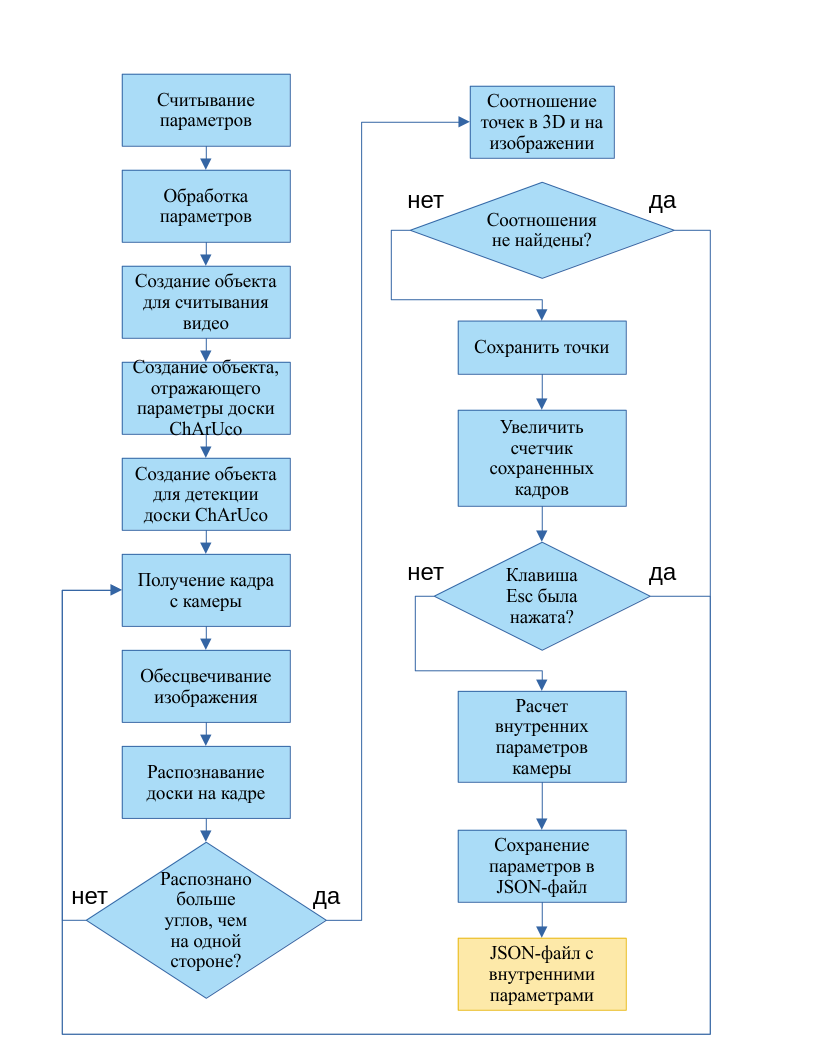
\includegraphics[width=0.95\textwidth]{images/block-schemes/intrinsics_scheme.png}
  \end{center}
  \caption{Блок-схема алгоритма калибровки камер}
  \label{fig:intrinsincs_block_scheme}
\end{figure}

Блок-схема алгоритма калибровки внутренних параметров камеры изображена на
рисунке \ref{fig:intrinsincs_block_scheme}.

Параметры нужны для того, чтобы с каждой из исполняемых програм было удобнее работать.
В каждой из них есть ряд параметров, которые можно указать при запуске. 
Они позволяют отлаживать код быстрее, а также позволяют выбирать нужные файлы,
камеры и другие вещи, которые могут меняться, "на ходу".
\par
\texttt{cam\_id} --- этот аргумент указывает идентификационный номер камеры.
На основании этого аргумента откроется устройство захвата через
\texttt{cv2.VideoCapture}. 
\listingsection{
../src/intrinsics_calibration.py
}{CAMID}

Также, есть два аргумента влияющих на формат названия:
\begin{itemize}
  \item \texttt{--no-error-name} --- если этот аргумент использован, то в
    названии выходного файла не будет указано значение ошибки перепроекции,
  \item \texttt{--no-frames-name} --- если этот аргумент использован, то в
    назыании выходного файла не будет указано количество записанных кадров для
    калибровки.
\end{itemize}
\listingsection{
../src/intrinsics_calibration.py
}{NAMEARGS}

Параметр \texttt{--output} хранит путь к выходному файлу и основу для его
названия, то есть, если этот аргумент имеет значение \texttt{calibration\_results/calibration\_L},
то в итоге выходной файл будет лежать в директории
\texttt{calibration\_results} и иметь название, например, \\
\texttt{calibration\_L\_frames=623\_error=1.5265531081871597.pkl}.
\listingsection{
../src/intrinsics_calibration.py
}{OUTPUTNAME}

Параметр \texttt{--capture\_json} хранит путь к файлу с параметрами создания
объекта захвата. Этот параметр нужен чтобы открывать объекты с одинаковыми
параметрами каждый раз.
\listingsection{
../src/intrinsics_calibration.py
}{CAPTUREJSON}

Параметр \texttt{--num-threads} указывает сколько потоков может использовать
OpenCV для проведения расчетов.
\listingsection{
../src/intrinsics_calibration.py
}{NUMTHREADS}

После введения аргументов, происходит их разбор и сохранение id камеры в
отдельную переменную:
\listingsection{
../src/intrinsics_calibration.py
}{PARSE}

Создается объект, отображающий параметры доски. Это нужно для того, чтобы
камера калибровалась на основе рельных известный расстояний. После этого, на основе
созданной доски, создается объект \texttt{cv2.aruco.CharucoDetector}, который
нужен для правильного распознаваия доски на изображении:
\listingsection{
../src/intrinsics_calibration.py
}{CREATECHARUCO}

Инициализируются переменные, необходимые для хранения точек, которые потребуются
для калибровки, также счетчик записанных кадров:
\listingsection{
../src/intrinsics_calibration.py
}{BASICINIT}

Открывается объект захвата, на основе заданных id камеры и файла конфигурации.
Функция \texttt{create\_caupture\_from\_json} определена в разделе с
вспомогательными функциями.
\listingsection{
../src/intrinsics_calibration.py
}{CREATECAPTURE}

После чего, начинается цикл захвата изображений, который идет до тех пор, пока
пользователь не нажмет на кнопку Escape.Последующий код будет
находиться внутри цикла \texttt{while True:}, пока я не укажу обратное.
\par
Сначала считывается изображение с объекта захвата и по переменной
\texttt{ret} проверяется, что изображение было успешно считано:
\listingsection{
../src/intrinsics_calibration.py
}{READFRAME}

После чего получается размер изображения, необходимый для калибровки:
\listingsection{
../src/intrinsics_calibration.py
}{GETSIZE}

Затем, изображение обесцвечивается, что необходимо для распознавания ChArUco доски:
\listingsection{
../src/intrinsics_calibration.py
}{DISCOLOR}

На grayscale-изображени распознается доска. Результатом работы этого кода
являются: 
\begin{itemize}
  \item набор углов клеток доски(\texttt{charuco\_corners})
  \item набор идентификаторов каждого из углов клеток(\texttt{charuco\_ids}),
  \item набор углов ArUco маркеров, расположенных на доске(\texttt{marker\_corners}),
  \item набор идентификаторов маркеров, расположенных на доске (\texttt{marker\_ids}).
\end{itemize}
После чего проверяется, был ли найден хотя бы один угол на доске.
В случае, когда не было найдено ни одного угла, исполнение программы
возвращается в начало цикла.
\listingsection{
../src/intrinsics_calibration.py
}{DETECT}

После этого, если углы и маркеры были обнаружены, они отрисовываются на
исходном изображении и результат обнаружения выводится на экран:
\listingsection{
../src/intrinsics_calibration.py
}{DISPLAY}

Далее проверяется, достаточно ли углов было найдено. 
Углов достаточно, когда их больше, чем максимальное возможное количество углов,
лежащих на одной прямой. Это условие гарантирует, что не все найденные углы
лежат на одной прямой. Если углов достаточно, то при помощи метода
\texttt{matchImagePoints} объекта доски \texttt{charuco\_board}, созданного
ранее, получаются:
\begin{itemize}
  \item координаты точек в пространстве --- \texttt{cur\_object\_points}, 
  \item координаты точек на изображении --- \texttt{cur\_image\_points}.
\end{itemize}
Эти переменные отображают соотвествие между координатами в трехмерном
пространстве и точками на изображении.
После чего, проверяется, получилось ли получить хотя бы одно соответствие между
точками. Если это условие выполняется, то счетчик сохраненных кадров
увеличивается на 1 и данные точки сохраняются для дальнейшей обработки. В
противном случае, исполнение возвращается в начало цикла.
\listingsection{
../src/intrinsics_calibration.py
}{SAVEPOINTS}

Далее, проверяется нажатие клавишы. Если была нажата клавиша Escape, то цикл прекращается.
\listingsection{
../src/intrinsics_calibration.py
}{WAITKEY}

На этом, считываение и обработка кадров заканчивается. Следующий код идет после цикла \texttt{while True}.

Как только пользователь нажал клавишу Escape, считываение кадров прекращается,
и закрываются все открытые для вывода изображений окна, а также освобождается
объект захвата \texttt{cap}.
\listingsection{
../src/intrinsics_calibration.py
}{CV2CLOSE}

Затем, вычисляются внутренние параметры камеры при помощи функции\\
\texttt{cv2.calibrateCamera}:

\listingsection{
../src/intrinsics_calibration.py
}{CALIBRATION}

Результатом работы этого кода являются:
\begin{itemize}
  \item \texttt{precision} --- дробное число, отражающее ошибку перепроекции с данными внутренними параметрами,
  \item \texttt{camera\_matrix} --- матрица камеры, о которой говорилось в \ref{sec:camera_model},
  \item \texttt{dist\_coeffs} --- коэффициенты искажений камеры.
\end{itemize}

Как только камера была откалибрована, формируется словарь с полученными данными, формируется название, и записывается в .pkl файл.
\listingsection{
../src/intrinsics_calibration.py
}{SAVEDATA}

    

\subsection{Калибровка положения}
\label{sec:position-calib}

Было описано как происходит проецирование точек на плоскость камеры. Однако, в
реальности не всегда удобно считать камеру центром СК. Поэтому, часто вводится
некая глобальная система координат. Назовем ее $O_{X_0Y_0Z_0}$. Эта система
координат связана с системой координат $C_{XYZ}$ через однородное
преобразование $T_{CO}$. Допустим, что вектор $\overline{A}_C \in \mathbb{R}^4$
представляет собой однородные координаты точки $A$ в СК $C_{XYZ}$, а вектор
$\overline{A}_O \in \mathbb{R}^4$ представляет собой координаты этой же точки в
СК $O_{X_0Y_0Z_0}$. Тогда:

\begin{equation}
    \overline{A}_C = T_{CO} \cdot \overline{A}_O.
\label{eqn:basic_matrix_tf}
\end{equation}
Если учесть~\eqref{eqn:pinhole_matrix_projection_real} и
подставить~\eqref{eqn:basic_matrix_tf} в него, получится:

\begin{equation}
\begin{gathered}
    \overline{a} = K \cdot \overline{A_C} = \\
    = K \cdot T_{CO} \cdot \overline{A_O}.
\end{gathered}
\label{eqn:full_projection}
\end{equation}
При этом, матрица однородного преобразования $T_CO$ состоит из двух частей:
\begin{equation}
\begin{gathered}
    T_CO = \left[ R \quad \vline \quad t \right] = \\
    = \left[
        \qquad R \qquad \vline \begin{pmatrix}
        x_t\\
        y_t\\
        z_t
    \end{pmatrix}
    \right],
\end{gathered}
\label{eqn:projection_matrix_tf}
\end{equation}
где $t$ --- вектор смещения, являющийся, по сути, просто положением доски, а $R$ ---
матрица поворота, полученная по формуле Родрига~\cite{opencv_rodrigues}:
\begin{equation}
\begin{gathered}
    R = \cos(\theta) I + (1 - \cos(\theta))r r^T + \sin(\theta) \begin{bmatrix}
         0   & -r_z & r_y\\
        r_z  & 0    & -r_x\\
        -r_y & r_x  & 0
    \end{bmatrix}.
\end{gathered}
\label{eqn:rodrigues_formula}
\end{equation}
При этом, вектор поворота $r$ является трехмерным вектором, норма которого равна
$\theta$ --- углу поворота, а сам вектор характеризует ось поворота.

Собирая вместе уравнения \eqref{eqn:rodrigues_formula},
\eqref{eqn:projection_matrix_tf}, \eqref{eqn:full_projection}, получим:
\begin{equation}
\begin{gathered}
    \overline{a} = K \cdot \left[R \quad \vline \quad t\right] \cdot \overline{A}_O = \\
    = P \cdot \overline{A}_O,
\end{gathered}
\label{eqn:proj_fomula_with_projection_matrix}
\end{equation}
где $P$ --- матрица проекции. У каждой камеры есть своя матрица проекции, через
которую можно определить как точка в пространстве будет спроецирована на
плоскость изображения.
Рассмотрим каждую составляющую, чтобы понять от чего зависит матрица проекции:
\begin{itemize}
    \item $K$ --- матрица внутренних характеристик, полученная в
    \ref{sec:camera_intrinsics_calibration}, она известна для камеры и не
    меняется для камеры, к которой относится,

    \item $R$ --- матрица поворота, при этом, эта матрица имеет лишь три
    независимых параметра, что видно из \ref{eqn:rodrigues_formula},

    \item $t$ --- вектор смещения.
\end{itemize}

Для калибровки положения необходимо найти матрицу проекции для каждой из
используемых камер. То есть нужно найти всего 6 неизвестных параметров. В OpenCV
это происходит при помощи ChArUco доски. На этой доске есть ряд характерных
точек, при этом, зная размер доски, легко расчитать расстояния между этими
точками. Таким образом, у нас есть относительные положения точек. Нам известны
их положения $\overline{A}_O$ и также нам известны их проекции на камере
$\overline{a}$. Нужно теперь подобрать такие значения $r$ и $t$, чтобы ошибка
перепроецирования $\overline{A}_O \rightarrow \overline{a}$ была минимальной.
Это делается методом наименьших квадратов в~\cite{opencv_charuco_pose}. Эту функцию
я использую в программе \texttt{calibration/orientation\_calibration.py} чтобы
получить положения доски ChArUco относительно камер. После чего, достаточно найти обратную к $T_{CO}$ матрицу, чтобы получить положение камер относительно центра $O$ системы координат $O_{X_0Y_0Z_0}$.

\subsection{Реализация калибровки положения}
Данная программа должна выполнять следующие вещи:
\begin{itemize}
  \item Открывать один или несколько источников видео,
  \item загружать внутренние параметры используемых камер,
  \item создать объекты параметров доски и детектора параметров,
  \item считывать кадр с каждого из открытых источников,
  \item распознавать доску ChArUco на кадрах,
  \item оценивать положение и поворот доски относительно камеры,
  \item сохранять положение доски в .pkl файл со словарем, содержащим данные о
    положении для каждой из указанных камер.
\end{itemize}

Блок схема данной программы изображена на рисунке \ref{fig:orientation_calibration_scheme}

\begin{figure}[h!]
  \begin{center}
    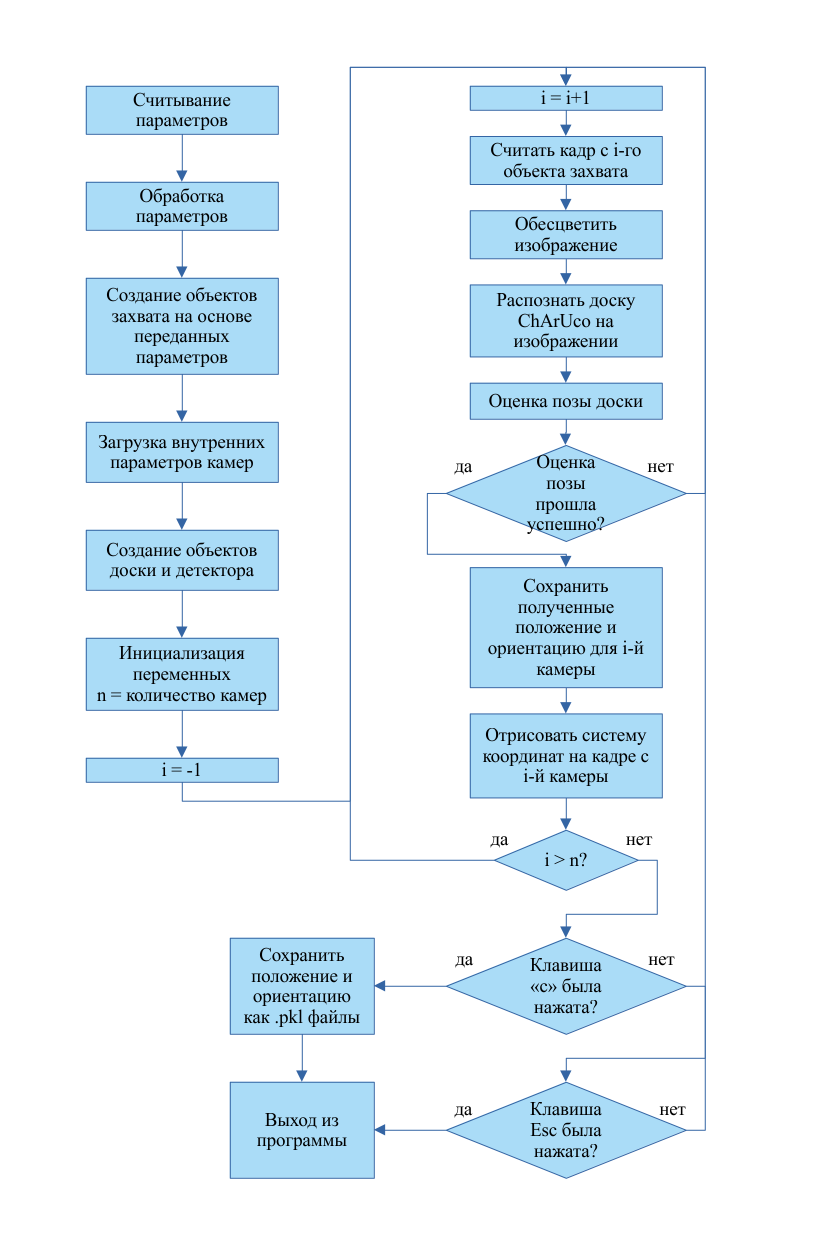
\includegraphics[width=0.95\textwidth]{images/block-schemes/orientation_scheme.png}
  \end{center}
  \caption{Блок-схема алгоритма калибровки положения камер}\label{fig:orientation_calibration_scheme}
\end{figure}

Калибровка положения реализована в файле \texttt{orientation\_calibration.py}.

У этой программы, как почти у любой другой в этом проекте, есть ряд аргументов
при запуске из коммандной строки. Перед тем, как программа начнет исполнение
алгоритма калибровки положения, в ней вводятся параметры, описанные дальше.

Параметр \texttt{input\_sources} хранит в себе видео или камеры, по которым
будет производиться калибровка.
\listingsection{
../src/orientation_calibration.py
}{INPUT_SOURCES}

Параметр \texttt{--intrinsics-files} хранит в себе пути к файлам с внутренними
параметрами камеры, которые были получены на предыдущем этапе калибровки.
\listingsection{
../src/orientation_calibration.py
}{INTRINSICS_FILES}

Параметр \texttt{--output} хранит путь где будут сохранены выходные файлы, а
так же префикс, с которого будут начинаться их названия.
\listingsection{
../src/orientation_calibration.py
}{OUTNAME}

Параметр \texttt{--separate} является флагом, если он использован, то данные
калибровки положения будут сохранены как два разных файла, в противном
случае, данные для двух камер будут сохранены в один файл.
\listingsection{
../src/orientation_calibration.py
}{SEPARATE}

Параметр \texttt{--display-scale} хранит в себе значение масштаба выводимых
изображений.
\listingsection{
../src/orientation_calibration.py
}{DISPLAY_SCALE}

После введения параметров проводится их разбор, сохранение списка источников
видео и масштаба, установка количества потоков и проверка наличия всех файлов
внутренних параметров.
\listingsection{
../src/orientation_calibration.py
}{INIT}

После чего:
\begin{itemize}
  \item проверяется, все ли переданные источники состоят из цифр, что означает, что они являются камерами,
  \item создается список, где будут храниться объекты захвата видео,
  \item на основе параметров либо открываются источники, не являющиеся
    камерами, либо открываются камеры через
    \texttt{create\_capture\_from\_json},
  \item созданные объекты захвата добавляются в созданный список.
\end{itemize}
\listingsection{
../src/orientation_calibration.py
}{PREP_CAMS}

Для корректной оценки положения камер, нужно загрузить их внутренные параметры.
Для этого, открывается каждый из указанных .pkl файлов, из словаря,
находящегося в нем, берутся матрица камеры и коэффициенты искажения.
\listingsection{
  ../src/orientation_calibration.py
}{LOAD_INTR}

Для детекции ChArUco доски, нужно создать объекты доски и детектора.
\listingsection{
  ../src/orientation_calibration.py
}{CHARUCO_SETUP}

После чего, проводится инициализация перед началом считывания. В ней
создаются: флаг успешного считывания, список полученных векторов поворота,
список полученных векторов положения и список внешних характеристик.
\listingsection{
  ../src/orientation_calibration.py
}{READ_INIT}

Затем, пока пользователь не даст комманду и пока считывание проходит
успешно, из каждого из созданных устройств захвата считывается кадр. Все
дальнейшие листинги кода происходят внутри цикла \texttt{while all\_ok:}, пока не
будет сказано обратное.
\listingsection{
  ../src/orientation_calibration.py
}{READ_FRAME}

Для корректной детекции доски, изображение нужно обесцветить.
\listingsection{
  ../src/orientation_calibration.py
}{DISCOLOR}

На обесцвеченном изображении созданный ранее детектор распознает доску и
возвращает найденные углы клеток доски, номера углов клеток, углы маркеров
на доске, номера маркеров.
\listingsection{
  ../src/orientation_calibration.py
}{DETECT}

Теперь при помощи функции \texttt{estimatePoseCharucoBoard} из библиотеки
OpenCV производится оценка положения доски на изображении. Эта функция
возвращает:
\begin{itemize}
  \item \texttt{ret} --- Флаг успешной оценки позы,
  \item \texttt{rvec} --- вектор поворота, который можно преобразовать в
    матрицу поворота при помощи формулы Родрига.
  \item \texttt{tvec} --- вектор смещения.
\end{itemize}
\listingsection{
  ../src/orientation_calibration.py
}{POSE_ESTIM}

Чтобы пользователь мог увидеть где находится центр координат, полученные
выше оси отрисовываются на изображении с камеры.
\listingsection{
  ../src/orientation_calibration.py
}{POSE_DISPLAY}

После чего, считывается клавиша с клавиатуры, чтобы пользователь мог
прекратить считываение кадров и сохранить данные, или прервать исполнение
программы.
\listingsection{
  ../src/orientation_calibration.py
}{CMD_INPUT}
Функция \texttt{save}:
\listingsection{
  ../src/orientation_calibration.py
}{SAVE_FUNC}

\section{Распознавание рук}
Нейросетевые методы распознавания не являются темой моей дипломной работы,
поэтому я не буду углубляться в то, как они работают, я буду использовать уже
готовую модель для выделения ключевых точек руки.

Сформулируем, что должно быть в этом модуле:
\begin{itemize}
  \item Считываение кадров с источника видео,
  \item предобработка, например, перевод в цветовое пространство RGB,
  \item распознавание точек на руке,
  \item опциональная отрисовка результатов детекции,
  \item возврат результатов детекции как массив точек на изображении.
\end{itemize}

В модуле распознавания рук описан класс \texttt{CaptureDetector}, который
открывает выбранный источник видео, на каждом полученном кадре находит
ключевые точки и возвращает их в определенном формате. Использование такой
структуры позволяет создать два отдельных объекта разпознавания для рук.
Благодаря этому, распознавание для каждой камеры может происходить параллельно,
или, например, во время отладки, можно запустить детекцию руки только для одной
камеры.

Для распознавания руки я решил использовать MediaPipe API от Google. Этот
программный интерфейс является довольно простым в работе и есть для языка
Python, который я использую.
MediaPipe имеет несколько режимов распознавания:
\begin{enumerate}
  \item на статичной картине --- \texttt{mp.tasks.vision.RunningMode.IMAGE},
  \item на декодированном видео --- \texttt{mp.tasks.vision.RunningMode.VIDEO},
  \item на потоке видео, в ``прямом эфире'' --- \texttt{mp.tasks.vision.RunningMode.LIVE\_STREAM}.
\end{enumerate}

Изначально, я предполгалал, что третий режим подойдет лучше всего, однако из-за
того, что документация на MediaPipe довольно ограничена и почти не описывает
этот режим, я решил использовать значительно лучше задокументированный режим
\texttt{VIDEO}. Этот режим распознает руку на каждом статичном изображении, как
и \texttt{IMAGE}, но, в отличие от него, в нем также используется отслеживание
движений между кадрами, что позволяет улучшить качество предсказаний модели.

\subsection{Класс \texttt{CaptureDetector}}
Распознавание рук происходит в классе \texttt{CaptureDetector}, описанном в файле \\ 
\texttt{detection/capture\_detector.py}
Этот класс используется как абстракция для выделения руки на изображении. У
этого класса есть две главные функции:
\begin{itemize}
  \item \texttt{\_\_init\_\_} --- инициализация,
  \item \texttt{process\_one\_frame} --- функция получения и обработки кадра.
\end{itemize}

\subsubsection{Инициализация \texttt{\_\_init\_\_()}}
Класс \texttt{CaptureDetector} при инициализации принимает на вход два аргумента:
\begin{itemize}
  \item \texttt{capture} --- уже созданный объект захвата
    \texttt{cv2.VideoCapture} для видео. Этот объект будет использоваться для
    получения кадров с камеры.
  \item \texttt{model\_path} --- путь к весам модели для распознавания.
\end{itemize}

В начале иницализации, переданный объект захвата сохраняется в поле класса
\texttt{cap}, а также из объекта захвата извлекаются ширина и высота изображения.
\listingsection{
  ../detection/capture_detector.py
}{INIT_CAP}

После этого создается переменная \texttt{base\_options}, хранящая в себе
базовые параметры программного интерфейса, а в частности параметры модели.
Создается объект \\\texttt{hand\_landmarker\_options}. Эта переменная нужна
только для того, чтобы строка с созданием объекта параметров детектора не была слишком
длинной. Для этого же создается переменная \texttt{running\_mode}.
Затем, создается поле \texttt{options}, которое хранит объект класса 
\\\texttt{ mp.tasks.vision.HandLandmarkerOptions}. Это поле отражает следующие
параметры распознавания:
\begin{itemize}
  \item путь к весам модели,
  \item режим распознавания,
  \item количество рук, которые модель может распознать на одном кадре.
\end{itemize}
После чего, наконец, создается сам объект детектора на основе введенных ранее
параметров и записывается в поле \texttt{landmarker}.
\listingsection{
  ../detection/capture_detector.py
}{INIT_TASK}
На этом заканчивается инициализация объекта \texttt{CaptureDetector}.

\subsubsection{Обработка изображения \texttt{process\_one\_frame}}
Для того, чтобы считать один кадр с объекта захвата и распознать ключевые
точки на нем, используется функция
\texttt{process\_one\_frame}.
Эта функция принимает на вход один аргумент --- \texttt{return\_frame}. Если
этот аргумент имеет истинное значение, то эта функция вместо кадра вернет
\texttt{None}.

В начале этой функции происходит 
\begin{enumerate}
  \item считывание изображения;
  \item проверка того, что изображение было считано;
  \item перевод из стандартного для OpenCV цветого пространства BGR в RGB,
    необходимое для корректного распознавания точек руки;
  \item создание объекта изображения \texttt{mediapipe.Image}, который
    используется в программном интерфейсе для распознавания.
\end{enumerate}
\listingsection{
  ../detection/capture_detector.py
}{FRAME_PREPROCESS}

Также, для улучшения распознавания, нужно знать время, в которое был считан кадр,
для чего используется метод \texttt{get} класса \texttt{VideoCapture}.
\listingsection{
  ../detection/capture_detector.py
}{GET_TIME}

После чего, с учетом временной метки кадра, получается результат детекции,
который, нужно заметить, является объектом класса \texttt{HandLandmarkerResult} 
из библиотеки MediaPipe.
\listingsection{
  ../detection/capture_detector.py
}{GET_DETECTION}

Затем, если функция должна вернуть кадр вместе с массивом распознанных точек,
то кадр переводится обратно в цветовое пространство BGR, необходимое для
корректного отображения изображения. Если же функция не должна возвращать
кадр, то его "указатель" обнуляется.
\listingsection{
  ../detection/capture_detector.py
}{FRAME_CONVERSION}

Также, перед тем как вытаскивать элементы из объекта результата детекции,
нужно проверить, было ли обнаужено хоть что-нибудь.
\listingsection{
  ../detection/capture_detector.py
}{DETECTION_CHECK}

В конце функции 
\begin{itemize}
  \item Выбирается результат для первой руки в списке распознанных рук,
  \item из результата детекции вытаскиваются координаты распознанных точек,
  \item полученные точки преобразуются из относительных координат на отрезке
    $\left[0; 1\right]$ в абсолютные координаты, измеряемые в пикселях,
  \item полученный список точек возвращается вместе с кадром.
\end{itemize}
\listingsection{
  ../detection/capture_detector.py
}{RESULT_PREPARATION}

В деструкторе класса закрывается модель для детекции, а также освобождаются объекты захвата.
\listingsection{
  ../detection/capture_detector.py
}{DESTRUCTOR}

\subsection{Пример запуска}
Пример того, как используется класс \texttt{CaptureDetector} написан в файле\\
\texttt{detection/run\_detection.py}.

Сначала, как обычно, вводятся аргументы, необходимые для более комфортной работы.
Для начала, указываются источники видео. Аргумент \texttt{source\_type} задает
тип источника: видео или поток с камеры. Он может иметь одно из двух значений:
cam или vid. Потом уже указываются источники в аргументе \texttt{sources}. Туда могут быть переданы пути к видео или номера камер в директории /dev. Аргумент \texttt{by-dev} должен быть указан в том случае, когда источники были указаны в формате /dev/video*.
\listingsection{
  ../src/run_detection.py
}{INPUT\_SRC\_ARG}

Также вводится пара аргументов, влияющих на производительность:
\begin{itemize}
  \item \texttt{buffer\_size} --- размер буффера, в который будут писаться еще не обработанные кадры,
  \item \texttt{framerate} --- целое число, описывающее целевое число кадров в секунду.
\end{itemize}
\listingsection{
  ../src/run_detection.py
}{PERF\_ARGS}

Затем, некоторые из указанных аргументов сохраняются в переменные.
\listingsection{
  ../src/run_detection.py
}{SAVE\_ARGS}

После этого, открываются объекты \texttt{cv2.VideoCapture} на основе введенных
аргументов. Сначала создается переменная \texttt{caps}, которая будет хранить в
себе список объектов захвата. Если указанный тип источник имеет значение cam,
то проверяется, был ли указан аргумент \texttt{by-dev}. Если нет, то она
переводит каждый аргумент из \texttt{sources} в целочисленный тип. Создаются
объекты \texttt{cv2.VideoCapture} и устанавливается размер буффера. В конце,
объект видеозахвата добавляется в созданный для них список.
\listingsection{
  ../src/run_detection.py
}{OPEN\_CAPS}

Также, нужно подготовить объекты распознавания рук. Для этого указывается путь
к весам модели, после чего для каждого из источников захвата создается объект
класса \texttt{CaptureDetector}, описанного ранее и сохраняются в список \texttt{detectors}.
\listingsection{
  ../src/run_detection.py
}{DETECTION}

Перед тем, как начать распознавание, происходит небольшая подготовка в виде
инициализации списков для объектов класса \texttt{Thread} и для кадров.
\listingsection{
  ../src/run_detection.py
}{CAPTURE_PREP}

Затем начинается цикл считывания и распознавания. Весь код, идущий ниже
находится внутри цикла \texttt{while}. В начале этого цикла сохраняется время
начала текущей итерации, что нужно для того, чтобы правильно расчитывать время
считывания кадров в соотвествии с целевым количеством кадров в секунду.
\listingsection{
  ../src/run_detection.py
}{WHILE}

Чтобы ускорить процесс распознавания и понизить время, требуемое для исполнения
одной итерации, используется многопоточная обработка. Для каждого из объектов в
списке \texttt{detectors} создается объект класса \texttt{Thread} для
исполнения функции обработки кадра и запускается.
\footnote{Данный способ является медленным, его можно улучшить создав потоки, на
которых детекторы непрерывно распознают руку.}
\listingsection{
  ../src/run_detection.py
}{RUN_DETECT}
Функция \texttt{run\_detector\_frame\_processing}, которую исполняют потоки
вызывает метод распознавания для одного кадра и отрисовывает результаты.
\listingsection{
  ../src/run_detection.py
}{FRAME_PROC}

После чего, работа каждого из потоков прекращается при помощи метода \texttt{Thread.join}
\listingsection{
  ../src/run_detection.py
}{GET_DETECT}

Чтобы проверить правильность распознавания, результаты выводятся на экран.
\listingsection{
  ../src/run_detection.py
}{DISPLAY}

В конце итерации получается время, которое она заняла. На основе этого времени
расчитывается, сколько нужно подождать для того, чтобы частота исполнения была
ближе к корректной. Ожидание происходит при помощи \texttt{cv2.waitKey},
которая также необходима для корректного вывода изображений на экран.
\listingsection{
  ../src/run_detection.py
}{SYNC}

Результат работы данной программы изображен на рисунках \ref{fig:run-detection-screenshots-1} и \ref{fig:run-detection-screenshots-2}.
\begin{figure}[!hp]
  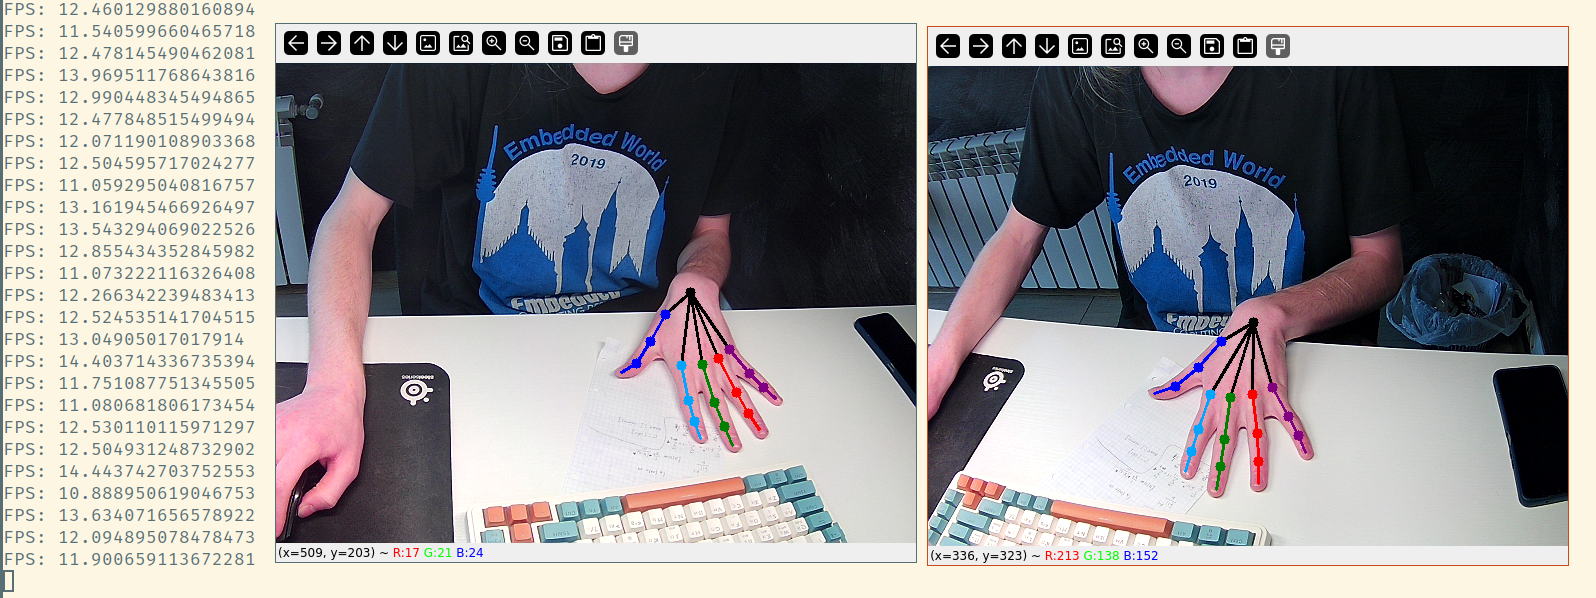
\includegraphics[width=\linewidth]{images/run-detection-screenshots/run-detection-1.png}
  \caption{Работа детектора на левой руке}\label{fig:run-detection-screenshots-1}
\end{figure}
\begin{figure}[!hp]
  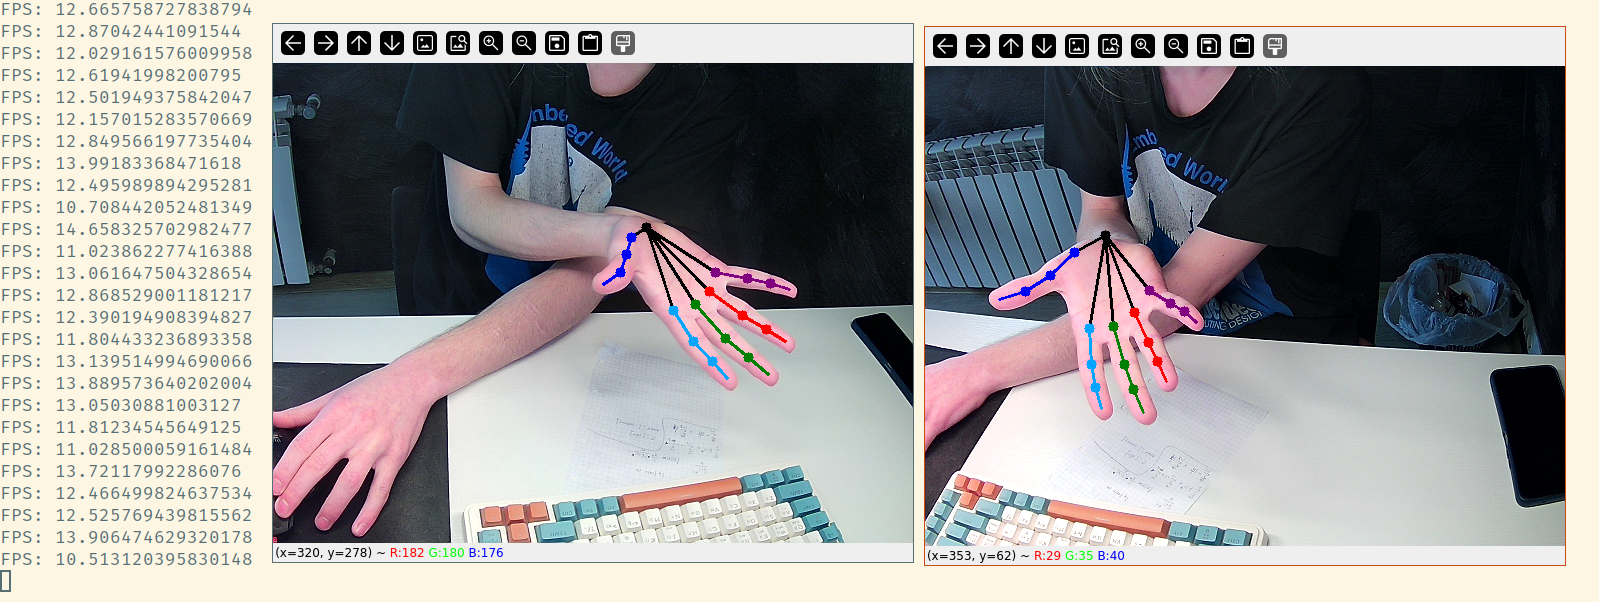
\includegraphics[width=\linewidth]{images/run-detection-screenshots/run-detection-2.png}
  \caption{Работа детектора на правой руке}\label{fig:run-detection-screenshots-2}
\end{figure}

\section{Получение позиции руки}
В рамках своей работы, я делаю систему, которая на основе данных с камер
распознает положение рук. Одним из методов получения координат точки на
основании ее проекций является триангуляция. \subsection{Постановка проблемы} В
\ref{sec:camera_model} была описана проекция на плоскость камеры. Очевидно, что
при этом происходит преобразование $\mathbb{R}^4 \rightarrow \mathbb{R}^3$, то
есть у нас теряется одна переменная. То есть для одной камеры получается
система линейных уравнений:
\begin{equation}
    \begin{pmatrix}
        x_a\\
        y_a\\
        z_a
    \end{pmatrix} = \begin{pmatrix}
        f X_A + Z p_x\\
        f Y_A + Z p_y\\
        Z_A 
    \end{pmatrix} = \underset{3 \times 4}{P} \begin{pmatrix}
        X_A\\
        Y_A\\
        Z_A\\
        1
    \end{pmatrix}.
\label{eqn:triangle_problem}
\end{equation}

Для определения координат в трехмерном пространстве, нужно найти $X_A$, $Y_A$,
$Z_A$, и при этом система \eqref{eqn:triangle_problem} содержит в себе 3
уравнения. Однако, если посмотреть на
уравнение~\eqref{eqn:pinhole_matrix_projection_real}, то несложно заметить, что
последнее уравнение в этой системе является вырожденным:
\begin{equation*}
    Z_A = Z_A
% \label{eqn:useless_triangle}
\end{equation*}
\par
Таким образом, для одной камеры имеется система из двух уравнений с тремя
неизвестными. Простейшим решением данной проблемы является добавление еще одной
камеры. Это позволит решить систему. В \cite{multiview_cv} и \cite{dlt_temugeb}
описана данная задача и ее решение. 
\subsection{Уравнения для одной камеры}
Система для $i$-й камеры выглядит так~\cite{multiview_cv, dlt_temugeb}:
\begin{equation}
    \overline{a}_i = \alpha P_i \overline{A}_O,
\label{eqn:general_dlt}
\end{equation}
где $\overline{a}_i$ --- вектор проекции точки $A$ на плоскость изображения
$i$-й камеры, $P_i$ --- матрица проекции для $i$-й камеры, а $\overline{A}_O$
--- координаты точки $A$ в глобальной системе координат $O_{X_0Y_0Z_0}$, а
$\alpha$ --- коэффициент, относящий длину вектора в правой части уравнения к
пиксельным координатам на изображении.

 Представим матрицу проекции как три четырехмерных вектора:
\begin{equation}
    P_i = \begin{bmatrix}
        \overline{p}_{i1}\\
        \overline{p}_{i2}\\
        \overline{p}_{i3}\\
    \end{bmatrix}
\end{equation}
Известно, что вектора в левой и правой частях уравнения параллельны, а значит,
их векторное произведение равно нулю:
\begin{equation}
    \begin{pmatrix}
        a_{xi}\\
        a_{yi}\\
        1
    \end{pmatrix} \times \begin{pmatrix}
        \overline{p}_{i1} \overline{A}_O\\
        \overline{p}_{i2} \overline{A}_O\\
        \overline{p}_{i3} \overline{A}_O
    \end{pmatrix} = \begin{pmatrix}
        a_{yi} \overline{p}_{i3} \overline{A}_O - \overline{p}_{i2} \overline{A}_O\\
        \overline{p}_{i1} \overline{A}_O - a_{xi} \overline{p}_{i3} \overline{A}_O\\
        a_{xi} \overline{p}_{i2} \overline{A}_O - a_{yi} \overline{p}_{i1} \overline{A}_O
    \end{pmatrix} = \begin{pmatrix}
        0\\
        0\\
        0
    \end{pmatrix}.
\label{eqn:full_cross_product}
\end{equation}
Упростим уравнение~\ref{eqn:full_cross_product}:
\begin{equation}
    \begin{pmatrix}
        a_{xi}\\
        a_{yi}\\
        1
    \end{pmatrix} \times \begin{pmatrix}
        \overline{p}_{i1} \overline{A}_O\\
        \overline{p}_{i2} \overline{A}_O\\
        \overline{p}_{i3} \overline{A}_O
    \end{pmatrix} = \begin{pmatrix}
        a_{yi} \overline{p}_{i3} - \overline{p}_{i2} \\
        \overline{p}_{i1} - a_{xi} \overline{p}_{i3} \\
        a_{xi} \overline{p}_{i2} - a_{yi} \overline{p}_{i1}
    \end{pmatrix} \overline{A}_O = \begin{pmatrix}
        0\\
        0\\
        0
    \end{pmatrix}.
\label{eqn:cross_product_one_camera}
\end{equation}

\subsection{Уравнения для двух камер}
\label{sec:two-cameras-eq}
Уравнение~\ref{eqn:cross_product_one_camera} описывает векторное
произведение векторов для одной камеры, теперь добавим вторую камеру:
\begin{equation}
\begin{gathered}
    \begin{pmatrix}
        a_{y1} \overline{p}_{13} - \overline{p}_{12} \\
        \overline{p}_{11} - a_{x1} \overline{p}_{13} \\
        a_{x1} \overline{p}_{12} - a_{y1} \overline{p}_{11}
    \end{pmatrix} \overline{A}_O = \begin{pmatrix}
        0\\
        0\\
        0
    \end{pmatrix}, \\
    \begin{pmatrix}
        a_{y2} \overline{p}_{23} - \overline{p}_{22} \\
        \overline{p}_{21} - a_{x2} \overline{p}_{23} \\
        a_{x2} \overline{p}_{22} - a_{y2} \overline{p}_{21}
    \end{pmatrix} \overline{A}_O = \begin{pmatrix}
        0\\
        0\\
        0
    \end{pmatrix}.
\end{gathered}
\label{eqn:two_cameras_cross_separate}
\end{equation}
Совместим в одну систему:
\begin{equation}
    \begin{pmatrix}
        a_{y1} \overline{p}_{13} - \overline{p}_{12} \\
        \overline{p}_{11} - a_{x1} \overline{p}_{13} \\
        a_{x1} \overline{p}_{12} - a_{y1} \overline{p}_{11}
        a_{y2} \overline{p}_{23} - \overline{p}_{22} \\
        \overline{p}_{21} - a_{x2} \overline{p}_{23} \\
        a_{x2} \overline{p}_{22} - a_{y2} \overline{p}_{21}
    \end{pmatrix} \overline{A}_O = \begin{pmatrix}
        0\\
        0\\
        0
    \end{pmatrix}.
\label{eqn:two_cameras_cross_joined}
\end{equation}
\subsection{Решение системы и минимизация шумов}
<<В реальном мире могут быть шумы, тогда система принимает вид:
\begin{equation}
M \overline{A}_{O} = w.
\label{eqn:noise_introduction}
\end{equation}
Нужно решить эту систему с минимальным шумом $w$\cite{dlt_temugeb}>>. Сделать это позволяет
SVD-разложение матрицы $M$:
\begin{equation}
    M \overline{A}_O = U S V^T \overline{A}_O.
\label{eqn:dlt-two-cameras-matrix}
\end{equation}
Чтобы прийти к минимальному шуму $w$, возьмем скалярное произведение левой и правой частей уравнения \eqref{eqn:noise_introduction}:
\begin{equation}
    w w^T =   \overline{A}_O^T V S U^T U S V^T \overline{A}_O.
\end{equation}
С учетом ортогональности матрицы $U: U^T U = I$:
\begin{equation}
    w w^T = \overline{A}_O^T V S S V^T \overline{A}_O = 
    \overline{A}_O^T V S^2 V^T \overline{A}_O.
\label{eqn:noise_squared_svd_simplify}
\end{equation}

Если взять в расчет ортогональность матрицы $V$ из-за свойств SVD-разложения,
то получим, что если умножить $i$-ю строку $v_i$ матрицы $V$ на
транспонированную матрицу $V^T$, то получится единичный вектор, где единичный
элемент стоит на $i$-й позиции:
\begin{equation}
\begin{gathered}
    v_i V^T = \begin{pmatrix}
        0 & \cdots & \underset{i-1}{0} & \underset{i}{1} & \underset{i+1}{0} & \cdots & 0
    \end{pmatrix} = e_i^T, \\
    V v_i^T = \begin{pmatrix}
        0 \\
        \vdots \\
        \underset{i-1}{0}\\
        \underset{i}{1}\\
        \underset{i+1}{0}\\
        \vdots\\
        0
    \end{pmatrix} = e_i.
\end{gathered}
\end{equation}
Тогда, если мы возьем $\overline{A}_O$ в системе
\eqref{eqn:noise_squared_svd_simplify} равным $i$-й строке матрицы $V$:
\begin{equation}
    w w^T = v_i^T V S^2 V^T v_i = s_i^2,
\end{equation}
где $s_i$ --- $i$-е сингулярное число в матрице $S$. Тогда достаточно взять $i$,
соответствующее минимальному сингулярному числу, в этом случае, квадрат 2-нормы
шума $w$ будет равен минимальному сингулярному числу. Шум минимизирован.

\subsection{Реализация}
Реализация триангуляции потребовала реализации нескольких элементов:
\begin{itemize}
  \item класс, который на основе взаимного положения камер будет расчитывать
    положение произвольной точки на изображении с обеих камер,
  \item класс, который будет визуализировать полученные точки,
  \item программа, которая совместит распознавание рук, загрузку
    откалиброванных параметров и визуализацию.
\end{itemize}

Класс для расчета положения должен инициализироваться параметрами камер, а
также их положением и ориентацией. У него также должен быть метод, у которого в
качестве аргументов будут координаты точек на изображении с первой камеры и со
второй. Он должен возвращать вектор этих точек в трехмерном пространстве. 

Модуль 3D визуализации должен создаваться на основе файлов конфигурации руки,
которые определяют цвета каждого из пальцев и связи между шарнирами в руке
человека. У него должен быть метод, который позволит создать трехмерный график,
на котором будут изображены все сочленения в руке человека. Также он должен
быть способен отрисовать оси координат по заданным направлениям каждой из осей.

Исполняемая программа помимо создания описанных выше классов также должна
создавать объект класса \texttt{CaptureDetector}, предварительно создав объекты
\texttt{VideoCapture}. После этого, должен быть цикл, в котором происходит
распознавание, триангуляция и опциональная отрисовка результата.

\subsection{Класс \texttt{Triangulator}}
Данный класс, реализованный в файле \texttt{positioning/triangulator.py}
используется для определия положения точки в трехмерном пространстве по ее
положению на изображениях с камеры. Он имеет следующие методы:
\begin{itemize}
  \item \texttt{\_\_init\_\_} --- метод инициализации;
  \item \texttt{create\_projection\_matrix} --- метод расчета матриц проекции,
    описанных в главе, про калибровку~\ref{sec:position-calib};
  \item \texttt{undistort\_image} --- метод для исправления искажений на
    изображении, основанный на внутренних параметрах камеры, про которые
    рассказывалось в главе про калибровку внутренних параметров~\ref{sec:camera_intrinsics_calibration};
  \item \texttt{undistort\_point} --- метод для исправления искажений только
    для одной точки, а не всего изображения, так же основанный на внутренних
    параметрах из~\ref{sec:camera_intrinsics_calibration};
  \item \texttt{get\_DLT\_matrix} --- метод для получения матрицы, описанная
    в~\ref{sec:two-cameras-eq} в уравнении \eqref{eqn:dlt-two-cameras-matrix};
  \item \texttt{triangulate} --- метод, который решает уравнение
    \eqref{eqn:dlt-two-cameras-matrix} методом, описанным в уравнениях
    \eqref{eqn:dlt-two-cameras-matrix}-\eqref{eqn:noise_squared_svd_simplify}.
\end{itemize}

\subsubsection{Инициализация}
Конструктор принимает на вход следующие аргументы:
\begin{itemize}
  \item \texttt{camera\_matrices} имеет тип \texttt{list[np.ndarray]} и
    содержит в себе матрицы камер, полученные на этапе калибровки камер
    \ref{sec:camera_intrinsics_calibration};
  \item \texttt{distortion\_coefficients} имеет тип \texttt{list[np.ndarray]} и содержит
    в себе коэффициенты искажения для каждой камеры;
  \item \texttt{cameras\_rvecs} имеет тип \texttt{list[np.ndarray]} и хранит в
    себе вектора поворота, полученные на этапе калибровки
    положения~\ref{sec:position-calib}каждой камеры;
  \item \texttt{cameras\_tvecs} имеет тип \texttt{list[np.ndarray]} и содержит
    в себе вектора смещения, также полученные на этапе калибровки положения;
  \item \texttt{image\_width} --- ширина изображения;
  \item \texttt{image\_height} --- высота изображения;
  \item \texttt{cameras\_extrinsics} --- другие внешние параметры, которые
    возвращает функция \\\texttt{cv2.calibrateCamera}.
\end{itemize}
\listingsection{
  ../positioning/triangulator.py
}{INIT_PARAMS}

В начале конструктора происходит инициализация полей класса.
\begin{itemize}
  \item В поле \texttt{camera\_matrices} сохраняются матрицы камер;
  \item в поле \texttt{dist\_coeffs} сохраняются коэффициенты искажений;
  \item в поле \texttt{rvecs} сохраняются вектора поворота;
  \item в поле \texttt{tvecs} сохраняюися вектора смещения; 
  \item поле \texttt{new\_cam\_matrices} инициализируется пустым списком, позже в
    него будут сохранены перерасчитанные матрицы камер.
  \item поле \texttt{undistortMaps} инициализируется пустым списком, позже в
    нем будут храниться объекты, которые нужны для исправления искажений;
  \item поле \texttt{projection\_matrices} инициализируется пустым списком,
    позже в нем будут храниться матрицы проекций камеры, о которых говорилось в
    главе про модель камеры~\ref{sec:camera_model};
  \item поле \texttt{extrinsics} инициализируется пустым списком.
\end{itemize}

После этого происходит перерасчет матриц камеры при помощи функции
\texttt{cv2.getOptimalNewCameraMatrix}. Новые матрицы камер добавляются в конец
поля \texttt{new\_cam\_matrices}. Также расчитываются "карты" перерасчета и
сохраняются в \texttt{undistortMaps}.
\listingsection{
  ../positioning/triangulator.py
}{MATR_INIT}

Затем происходит создание матриц проекций для каждой из камер на основе
полученных матриц камеры, векторов смещения и векторов поворота.
\listingsection{
  ../positioning/triangulator.py
}{PROJ_MATR_INIT}
Функция \texttt{create\_projection\_matrix} просто преобразует и умножает
матрицы так, чтобы на выходе получилась матрица однородного преобразования.
\listingsection{
  ../positioning/triangulator.py
}{PROJ_MATR_METHOD}

\subsubsection{Триангуляция}
Главным методом класса \texttt{CameraTriangulator} является \texttt{triangulate}.
Его блок-схема изображена на рисунке \ref{fig:triangulation_scheme}.
\begin{figure}[h!]
  \begin{center}
    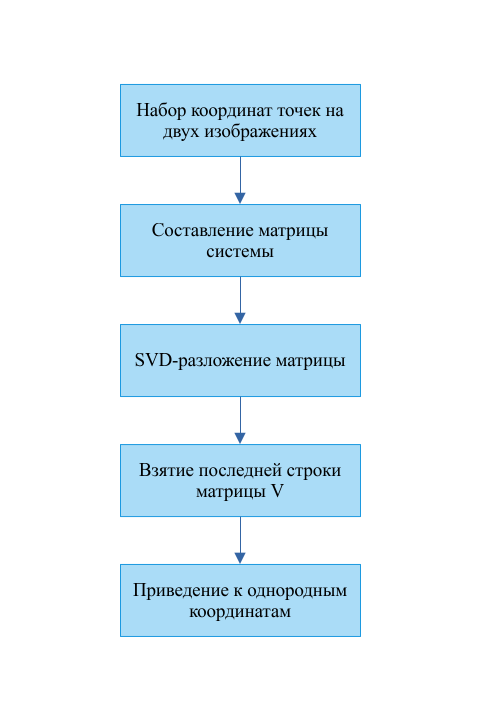
\includegraphics[width=0.6\textwidth]{images/block-schemes/triangulation_scheme.png}
  \end{center}
  \caption{Блок-схема алгоритма триангуляции точки}\label{fig:triangulation_scheme}
\end{figure}

Этот метод принимает на вход список из двух векторов: координат точки на
изображении с первой камеры и со второй.
Сначала, создается матрица $M$, описанная в уравнении
\eqref{eqn:dlt-two-cameras-matrix}. 
\listingsection{
  ../positioning/triangulator.py
}{GET_DLT}
Рассмотрим метод \texttt{get\_DLT\_matrix}. Этот метод принимает на вход список
координат точек на нескольких камер. Для каждой из этих координат составляется
матрица, как было описано в уравнении \eqref{eqn:cross_product_one_camera}.
Затем в этом методе происходит слияние этих матриц в одну, как было описано при
переходе от \eqref{eqn:two_cameras_cross_separate} к
\eqref{eqn:two_cameras_cross_joined}.

Затем, происходит SVD-разложение полученной матрицы, что является одним из
способов снижения шума.
\listingsection{
  ../positioning/triangulator.py
}{SVD}

Из-за того, как происходит SVD-разложение в библиотеке NumPy, возвращается не
матрица $V$, а ее Эрмитово сопряженная матрица $V^H$. То есть, если в матрице
$V$ есть комплексные числа, то матрица $V^H$ являет собой транспонированную
матрицу $V$, где вместо изначальных комплексных чисел стоят их
комплексно-сопряженные~\cite{numpy_svd}. Также, эта функция возвращает
сингулярные числа в порядке убывания, из чего следует, что желаемый вектор
лежит в последнем столбце матрицы $V^H$. Возьмем этот вектор и приведем к вектору в
нормальных, координатах, разделив на его последний элемент. Так получается
искомый вектор положения.
\listingsection{
  ../positioning/triangulator.py
}{SVD_RES}

\subsection{Запуск расчета 3D координат руки}
Программа, которая запускает позиционирование реализована в файле\\
\texttt{run\_hand\_positioning.py}.

\subsubsection{Входные аргументы}
Как и в любом другом исполняемом файле, эта программа начинается с того, что
вводятся аргументы. Здесь их особо много в силу того, что в этой программе
задействуется множество модулей, у каждого из которых есть параметры.
Определение аргументов здесь происходит в отдельной функции
\texttt{parse\_args}.
Первым делом вводится аргумент \texttt{cam\_ids}, принимающий два аргумента
типа int, которые указывают на номера камер в /dev/video*.
\listingsection{
  ../src/run_hand_positioning.py
}{CAM_IDS}

Аргумент \texttt{capture\_json} является частью универсальной кофигурации
проекта, он указывает на JSON-файл, где хранятся параметры текущих камер. Нужен
для того, чтобы все исполняемые программы открывали камеры одинаково.
\listingsection{
  ../src/run_hand_positioning.py
}{CAPTURE_JSON}

После этого, вводятся аргументы \texttt{camera-intrinsics} и
\texttt{orientation}, которые хранят пути к файлам внутренних параметров,
положения и ориентации.
\listingsection{
  ../src/run_hand_positioning.py
}{CAMERA_PARAMETERS}

Аргумент \texttt{num-threads} принимает значение потоков, которые будут
выделены OpenCV для расчетов.
\listingsection{
../src/run_hand_positioning.py
}{N_THREADS}

Вводятся параметры вывода видео на экран. Если параметр \texttt{show-video}
указан, то видео с камер будет выведено. Параметр \texttt{display-scale} хранит
значение масштаба изображений. 
\listingsection{
  ../src/run_hand_positioning.py
}{ARGS_VIDEO}

Последний параметр --- \texttt{show-hands} --- указывает, нужно ли
визуализировать результаты работы в виде 3D графика.
\listingsection{
  ../src/run_hand_positioning.py
}{ARGS_HANDS}

\subsubsection{Исполняемый код}
Исполнение этой программы начинается с того, что аргументы считываются, а
некоторые из них сохраняются в переменные.
\listingsection{
  ../src/run_hand_positioning.py
}{SAVE_ARGS}

После этого создаются объекты захвата \texttt{cv2.CaptureDetector} и
распознавания \texttt{CaptureDetector}.
\listingsection{
  ../src/run_hand_positioning.py
}{DET_CAPS}

Создается объект класса \texttt{CameraTriangulator}, который будет проводить
реконструкцию положения точек. 
\listingsection{
  ../src/run_hand_positioning.py
}{TRI_CREATE}

Если был указан параметр \texttt{show-hands}, то также создается объект класса
\texttt{Visualizer3D}, который используется для отображения результатов
триангуляции на трехмерном графике.
\listingsection{
  ../src/run_hand_positioning.py
}{VIZ_CREATE}

Создается объект класса \texttt{GripperConverter}.
\listingsection{
  ../src/run_hand_positioning.py
}{GRIP_CONV}

Затем инициализируются переменные, которые будут использоваться в цикле далее.
Также для того, чтобы более корректно отображать оси на изображении, вводятся
новые вектора поворотов \texttt{new\_rvecs} для каждой из двух камер. Это нужно
из-за того, что для доски ChArUco оси определяются так, что ось Z смотрит "вниз".
\listingsection{
  ../src/run_hand_positioning.py
}{INIT}

Основные расчеты происходят внутри цикла \texttt{while True}. Весь код,
приведенный далее будет находиться внутри этого цикла, пока не будет указано
обратное. В начале каждой итерации сохраняется время ее начала, что нужно для
того, чтобы оценить быстродействие. Для каждого из объектов
\texttt{CaptureDetector} просиходит обработка кадра и сохраняется в список с
распознанными точками и кадрами.
\listingsection{
  ../src/run_hand_positioning.py
}{READ}

Затем происходит проверка того, что рука была распознана на обеих камерах. Если
это не так, то итерация начинается заново.
\listingsection{
  ../src/run_hand_positioning.py
}{BOTH_DETECTED}

Для каждой из распознанных точек происходит триангуляция и ее результат
записывается в список \texttt{points3d}.
\listingsection{
  ../src/run_hand_positioning.py
}{RUN_TRI}

Затем происходит получение ориентации руки при помощи модуля
\texttt{GripperConverter}. Это опциональный шаг, ибо визуализатор может не
отрисовывать оси, если вместо них был передан \texttt{None}.
\listingsection{
  ../src/run_hand_positioning.py
}{GET_ORIENT}

Потом, если указан параметр \texttt{show-hands}, расчитанные положения точек визуализируются при помощи класса
\texttt{Visualizer3D}. О нем рассказано в секции про визуализацию.
%todo{описание класса визуализации.}
\listingsection{
  ../src/run_hand_positioning.py
}{UPDATE_VIZ}

Также, если указан параметр \texttt{show\_video}, то на каждом из кадров
будут отрисованы оси системы координат, относительно которой расчитвается
положение и распознанные точки руки.
\listingsection{
  ../src/run_hand_positioning.py
}{DISPLAY}

В конце итерации замеряется время и печатается количество кадров в секунду.
Также, ожидается нажатие клавиши Escape. Если она была нажата, то цикл
прерывается.
\listingsection{
  ../src/run_hand_positioning.py
}{TIME}

На этом код внутри цикла \texttt{while} заканчитвается. После того, как цикл
завершил исполнение, объекты захвата освобождаются, а все открытые окна для
отрисовки кадров закрываются. 
\listingsection{
  ../src/run_hand_positioning.py
}{FINISH}

\subsection{Визуализация}
Для того, чтобы визуализировать руку в трехмерном пространстве, был написан
класс \texttt{Visualizer3D}. Его реализация находится в файле
\texttt{visualizer\_3d.py}.
Этот класс работает так, что при его создании происходит инициализация, а
затем он только обновляется при помощи метода \texttt{update}.

Его конструктор  --- \texttt{\_\_init\_\_} ---  создает объект графика, на
котором будут рисоваться токи, устанавливает параметры для для этого графика, а
также загружает конфигурацию для цветов и связей между ключевыми точками руки.
\listingsection{
  ../utils/visualizer_3d.py
}{INIT}
 В конце инициализации вызывается метод \texttt{set\_axes}. Этот метод
  расставляет названия осей и пределы в которых будут рисоваться полученные точки.
\listingsection{
../utils/visualizer_3d.py
}{SET_AXES}

Главный метод этого класса --- \texttt{update\_points}. Рассмотим его входные аргументы.
\begin{itemize}
  \item \texttt{joint\_coordinates} --- список из точек в трехмерном
    пространстве, описывающих руку;
  \item \texttt{axes} --- набор из трех векторов, описывающих инструментальную
    систему координат;
  \item \texttt{axes\_center} --- трехмерный вектор, описывающий положение
    центра инструментальной системы координат;
  \item \texttt{pause} --- параметр, указывающий на сколько секунд стоит
    остановить отрисовку перед следующим вызовом метода
    \texttt{update\_points};
  \item \texttt{camera} --- набор трехмерных векторов, описывающих положение
    камер в выбранной системе координат;
  \item \texttt{camera\_colors} --- параметр, который задает цвет, которым
    будут отрисовываться камеры.
\end{itemize}
\listingsection{
../utils/visualizer_3d.py
}{UPDATE_PARAMETERS}

Перед тем как перейти к отрисовке заданных точек, нужно очистить то, что уже
было нарисовано.
\listingsection{
  ../utils/visualizer_3d.py
}{CLEAR}

В начале, если они были переданы, рисуются точки руки при помощи метода
\texttt{draw\_hand}.
\listingsection{
  ../utils/visualizer_3d.py
}{DRAW_HAND_UPDATE}
Рассмотрим метод \texttt{draw\_hand}, который для этого используется.
Он принимает на вход набор точек, который характеризуют ключевые точки руки.
После чего, в цикле \texttt{for} рисуются связи между всем точками, указанными
в словарях, загруженных на этапе иницализации.
\listingsection{
../utils/visualizer_3d.py
}{DRAW_HAND}

После этого, если были переданы ориентация и положение выходного звена, то они
рисуются при помощи метода \texttt{draw\_coordinates}.
\listingsection{
  ../utils/visualizer_3d.py
}{DRAW_ORIENTATION}
Метод \texttt{draw\_coordinates} просто рисует линии, исходящие из заданной
точки, вдоль каждого из векторов, характреризующих ориентацию.
\listingsection{
  ../utils/visualizer_3d.py
}{DRAW_COORDINATES}

Затем рисуются точки камер, если таковые были переданы.
\listingsection{
../utils/visualizer_3d.py
}{DRAW_CAMERAS}

В конце метода \texttt{update\_points} происходит установка параметров оси и
пауза, необходимая для корректной работы отрисовщика.
\listingsection{
  ../utils/visualizer_3d.py
}{SET_AXES}


\section{Приведение руки к захвату манипулятора}
Этот шаг не имеет какого-то определенного устоявшегося подхода. Я для
себя выделил три возможных метода приведения рук:
\begin{enumerate}
    \item Простой метод, основанный на большом и указательном пальцах,
    \item эвристический метод,
    \item нейросетевой подход.
\end{enumerate}
О простом методе будет рассказано чуть позже, а пока я расскажу про методы,
которые не попали в мою работу.

Эвристический метод основывается на том, чтобы взять несколько часто
встречающихся способов взять предмет, рассмотреть характерные черты для каждого
и реализовать функцию, которая оценит близость текущей конфигурации к каждому
из вариантов взятия предметов. Преимущество метода --- высокий уровень контроля
результатов, ведь функция вводится "вручную". Среди недостатков этого метода
находится то, что неизвестно как именно вводить функцию и при введении можно
упустить какие-либо факторы или не учесть какой-то из вариантов захвата.

Нейросетевой метод близок к эвристическому, но основан на том, чтобы
натренировать модель, которая по входному массиву точек будет определять точку
схвата. По сути своей этот метод идентичен эвристическому, только функция и
способы захвата находятся при помощи машинного обучения, а не вводятся
человеком. Для тренировки модели, однако, нужен большой размеченный датасет,
где на каждой конфигурации точек отмечена точка захвата.

Преимуществом данного метода перед остальными является потенциально высокая
универсальность. При достаточно обширном датасете, этот метод может обеспечить
работу с любыми методами захвата, которые были представлены в наборе данных,
что сильно лучше чем простой метод. Помимо этого, он имеет возможность
обеспечить сильно лучшую точность, нежели простой метод, так как степень
раскрытия захвата не определяется какими-то заранее заданными точками, а
зависит от объекта. При правильном датасете, модель может быть способна это
учесть.

У этого метода, однако, есть два главных недостатка: затраты по времени и по
ресурсам. Сбор качественного набора данных и его разметка может занять очень
многое время. К тому же, не совсем ясно как именно размечать, для этого должен
уже быть какой-то способ определения расстояния, на которое нужно раскрыть
захват. Помимо сложностей со сбором набора данных, также для того, чтобы
обучение модели закончилось в сколь угодно разумные сроки, необходимы
вычислительные мощности, которых у меня нет.

\subsection{Простой метод}
\label{sec:gripper_basic_method}
Этот метод предполагает, что человек, использующий систему, берет все предметы
используя лишь указательный и большой палец. 
Для того, чтобы реализовать этот метод достаточно взять 4 точки:
\begin{itemize}
  \item точку $\overline{T_b}$, в которой начинается большой палец,
  \item точку $\overline{T_e}$, в которой кончается большой палец,
  \item точку $\overline{I_b}$, в которой начинается указательный палец,
  \item точку $\overline{I_e}$, в которой кончается указательный палец.
\end{itemize}
Координаты каждой из этих точек представлены как трехмерные вектора.

Сначала найдем точку $\overline{B}$, которая лежит между начальными точками:
\begin{equation}
  \overline{B} = \frac{\overline{T_b} + \overline{I_b}}{2}.
\end{equation}
Эта точка нужна для того, чтобы определить ориентацию выходного звена и
провести ось $Z$ инструментальной системы координат.
Затем найдем точку $\overline{E}$, лежащую между конечными точками:
\begin{equation}
  \overline{E} = \frac{\overline{T_e} + \overline{I_e}}{2}.
\end{equation}
Точка $\overline{E}$ характеризует положение захвата, а также служит для
построения инструментальной системы координат.

Тогда, плоскость захвата будет определяться тремя точками: $T_e, I_e, B$, а ось
$Z$ инструментальной системы координат лежит вдоль вектора $\overline{E} -
\overline{B}$. Ось $X$ можно найти следующим образом:
\begin{equation}
  X = (\overline{I_e} - \overline{B}) \times (\overline{T_e} - \overline{B}).
  \label{eqn:instumental_x_axis}
\end{equation}
При таком способе нахождения оси $X$, она будет направлена из тыльной стороны
ладони для правой руки.
Ось $Y$ для любой правой тройки векторов тоже можно найти через векторное произведение:
\begin{equation}
  Y = Z \times X.
  \label{eqn:instumental_y_axis}
\end{equation}
Таким образом, из набора точек получается ориентация и положение выходного
звена.


Визуализация этого метода на кадрах с камер изображена на рисунке
\ref{fig:basic_gripping}. Работа этого метода и отображение результата в
трехмерных координатах изображены на рисунке \ref{fig:basic_gripper_work}.
\begin{figure}[h!]
    \centering
    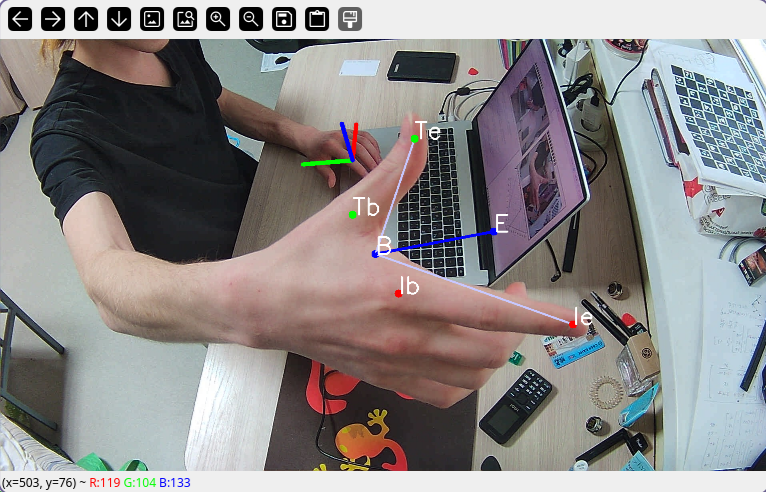
\includegraphics[width=0.66\textwidth]{images/gripper-conversion/gripper-conversion-close-1.png}\\
    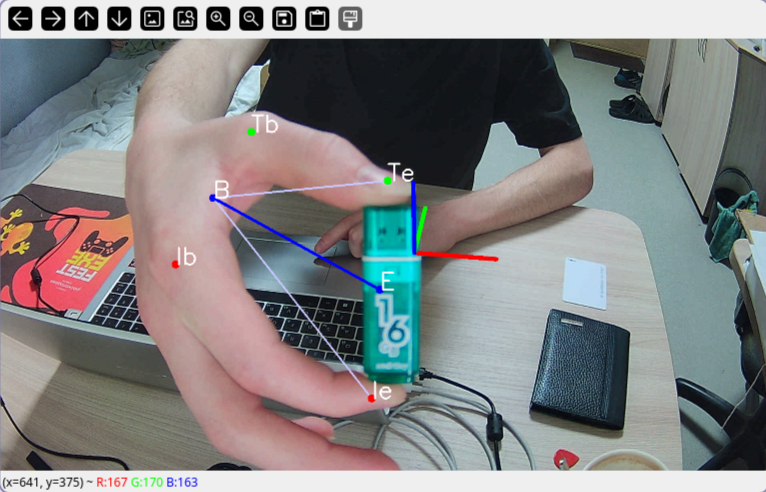
\includegraphics[width=0.66\textwidth]{images/gripper-conversion/gripper-conversion-close-2.png}\\
    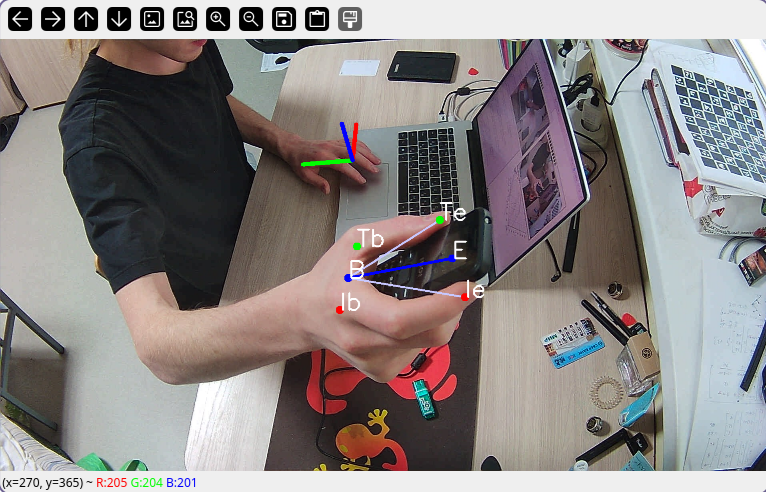
\includegraphics[width=0.66\textwidth]{images/gripper-conversion/gripper-conversion-close-3.png}\\
    \caption{Визуализация точки захвата}
~\label{fig:basic_gripping}
\end{figure}

\begin{figure}
  \begin{center}
    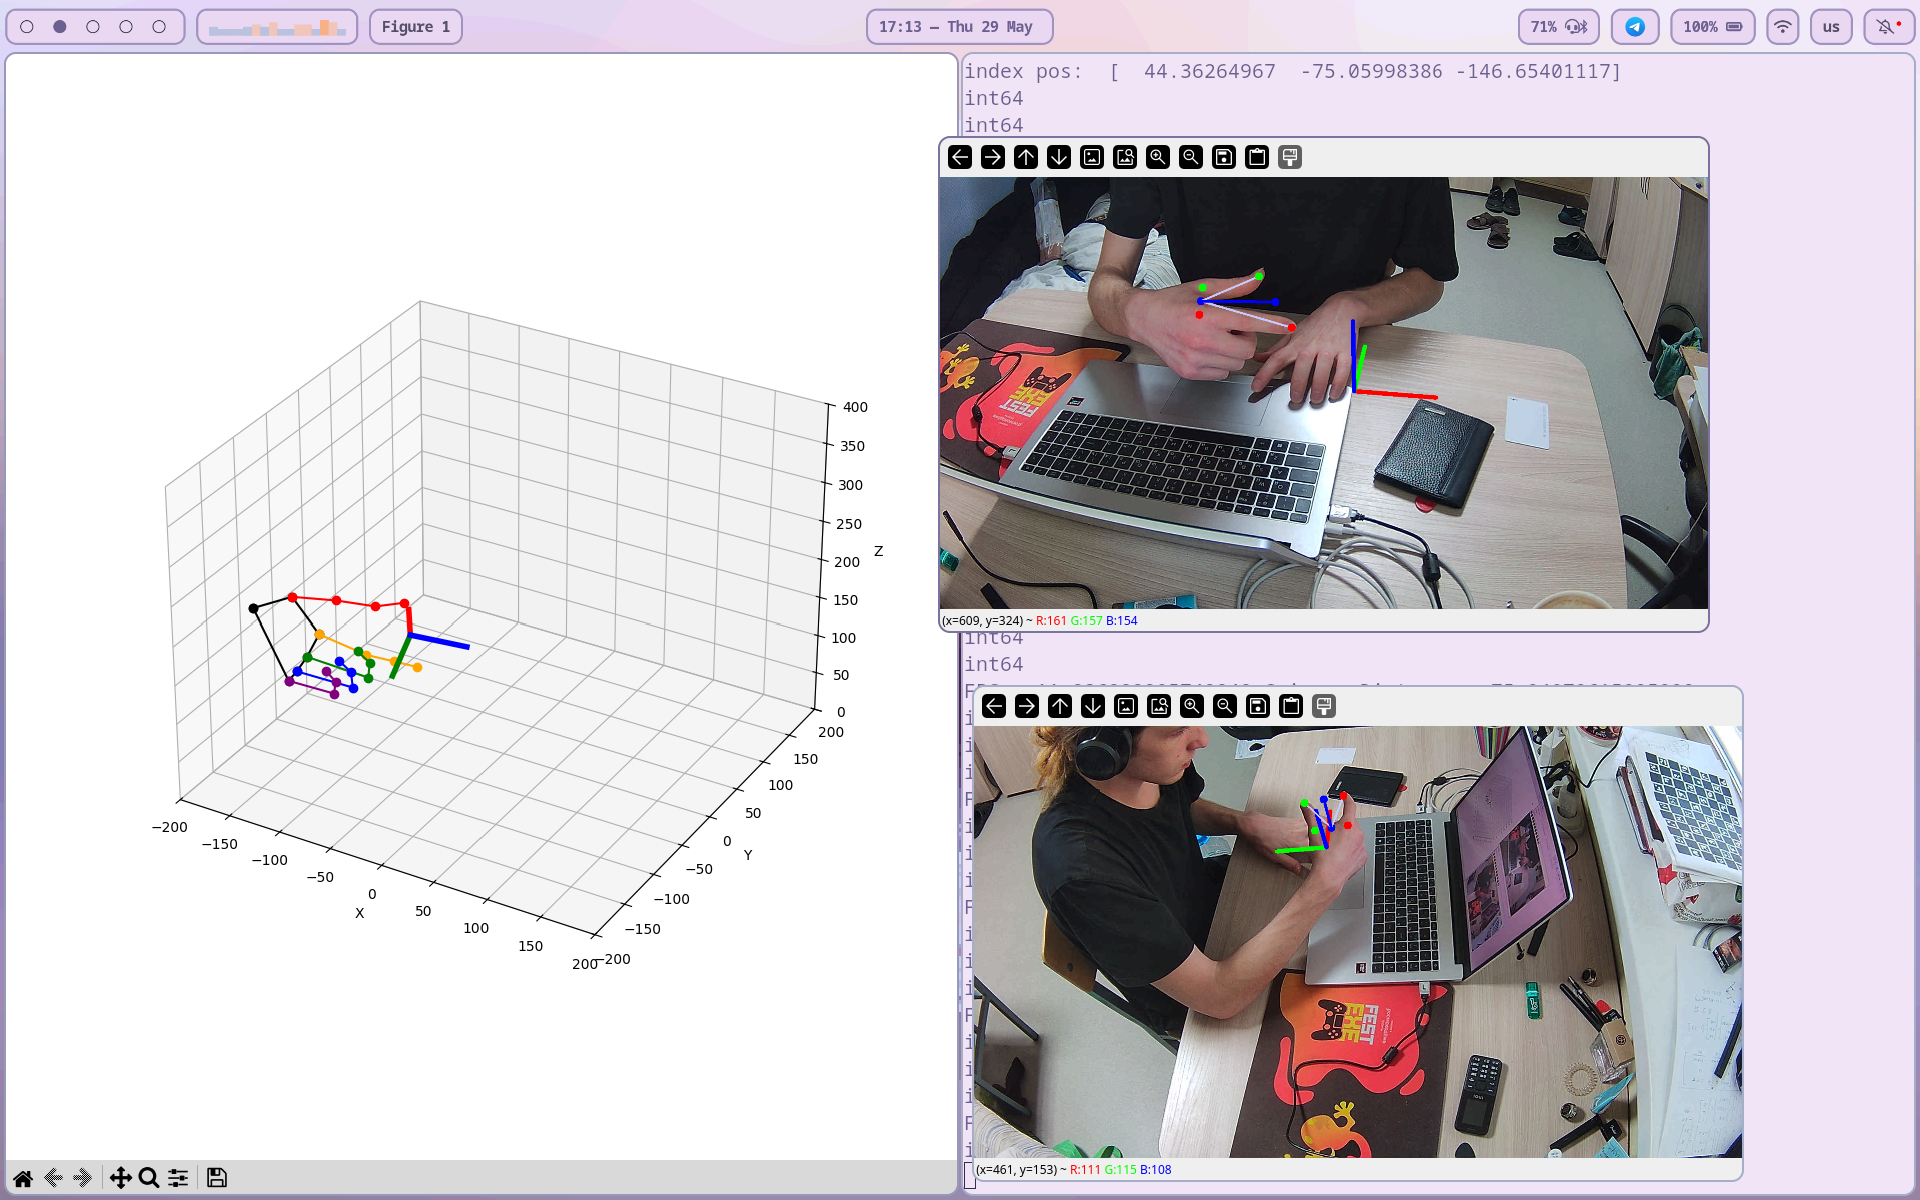
\includegraphics[width=0.7\textwidth]{images/gripper-conversion/gripper-conversion-1.png}\hfill
    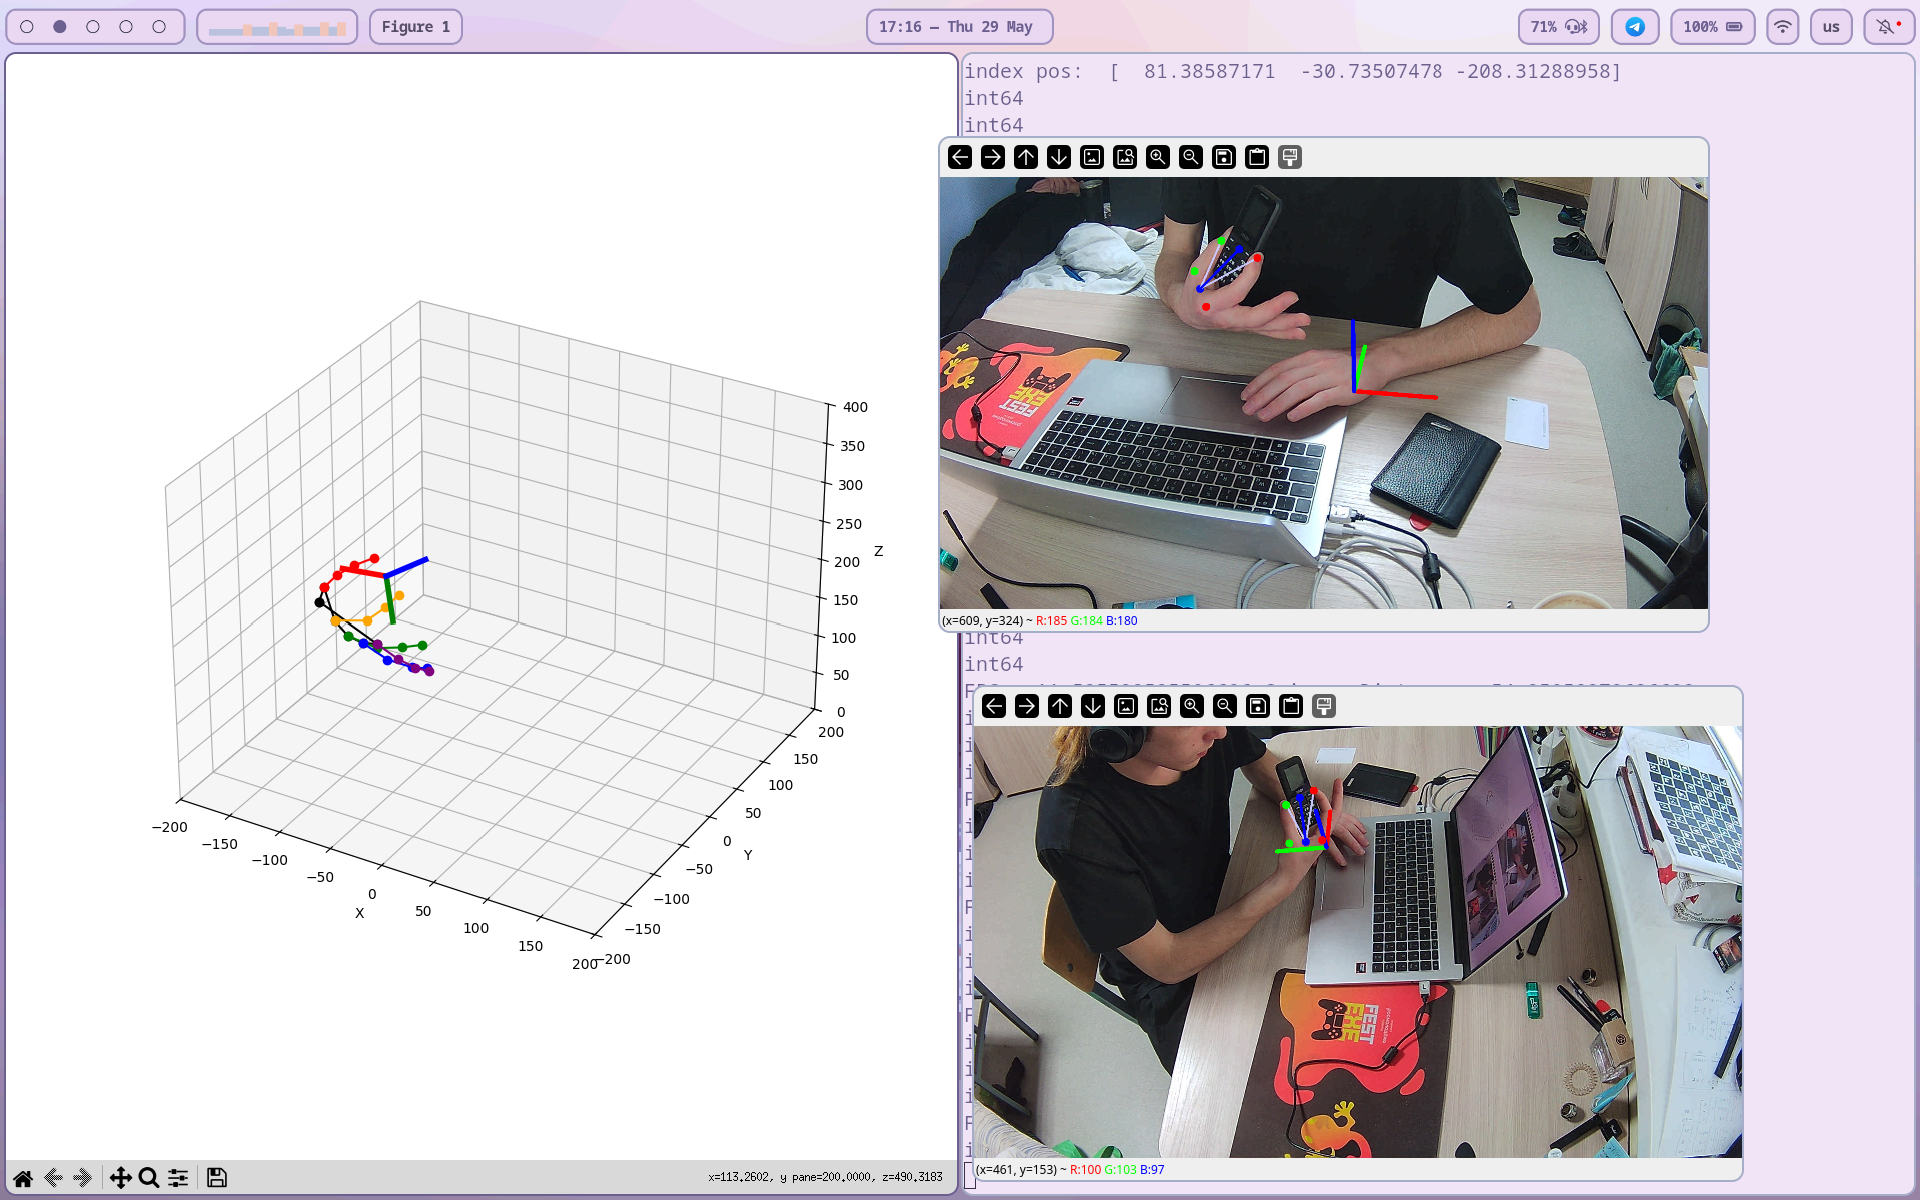
\includegraphics[width=0.7\textwidth]{images/gripper-conversion/gripper-conversion-2.png}\hfill
    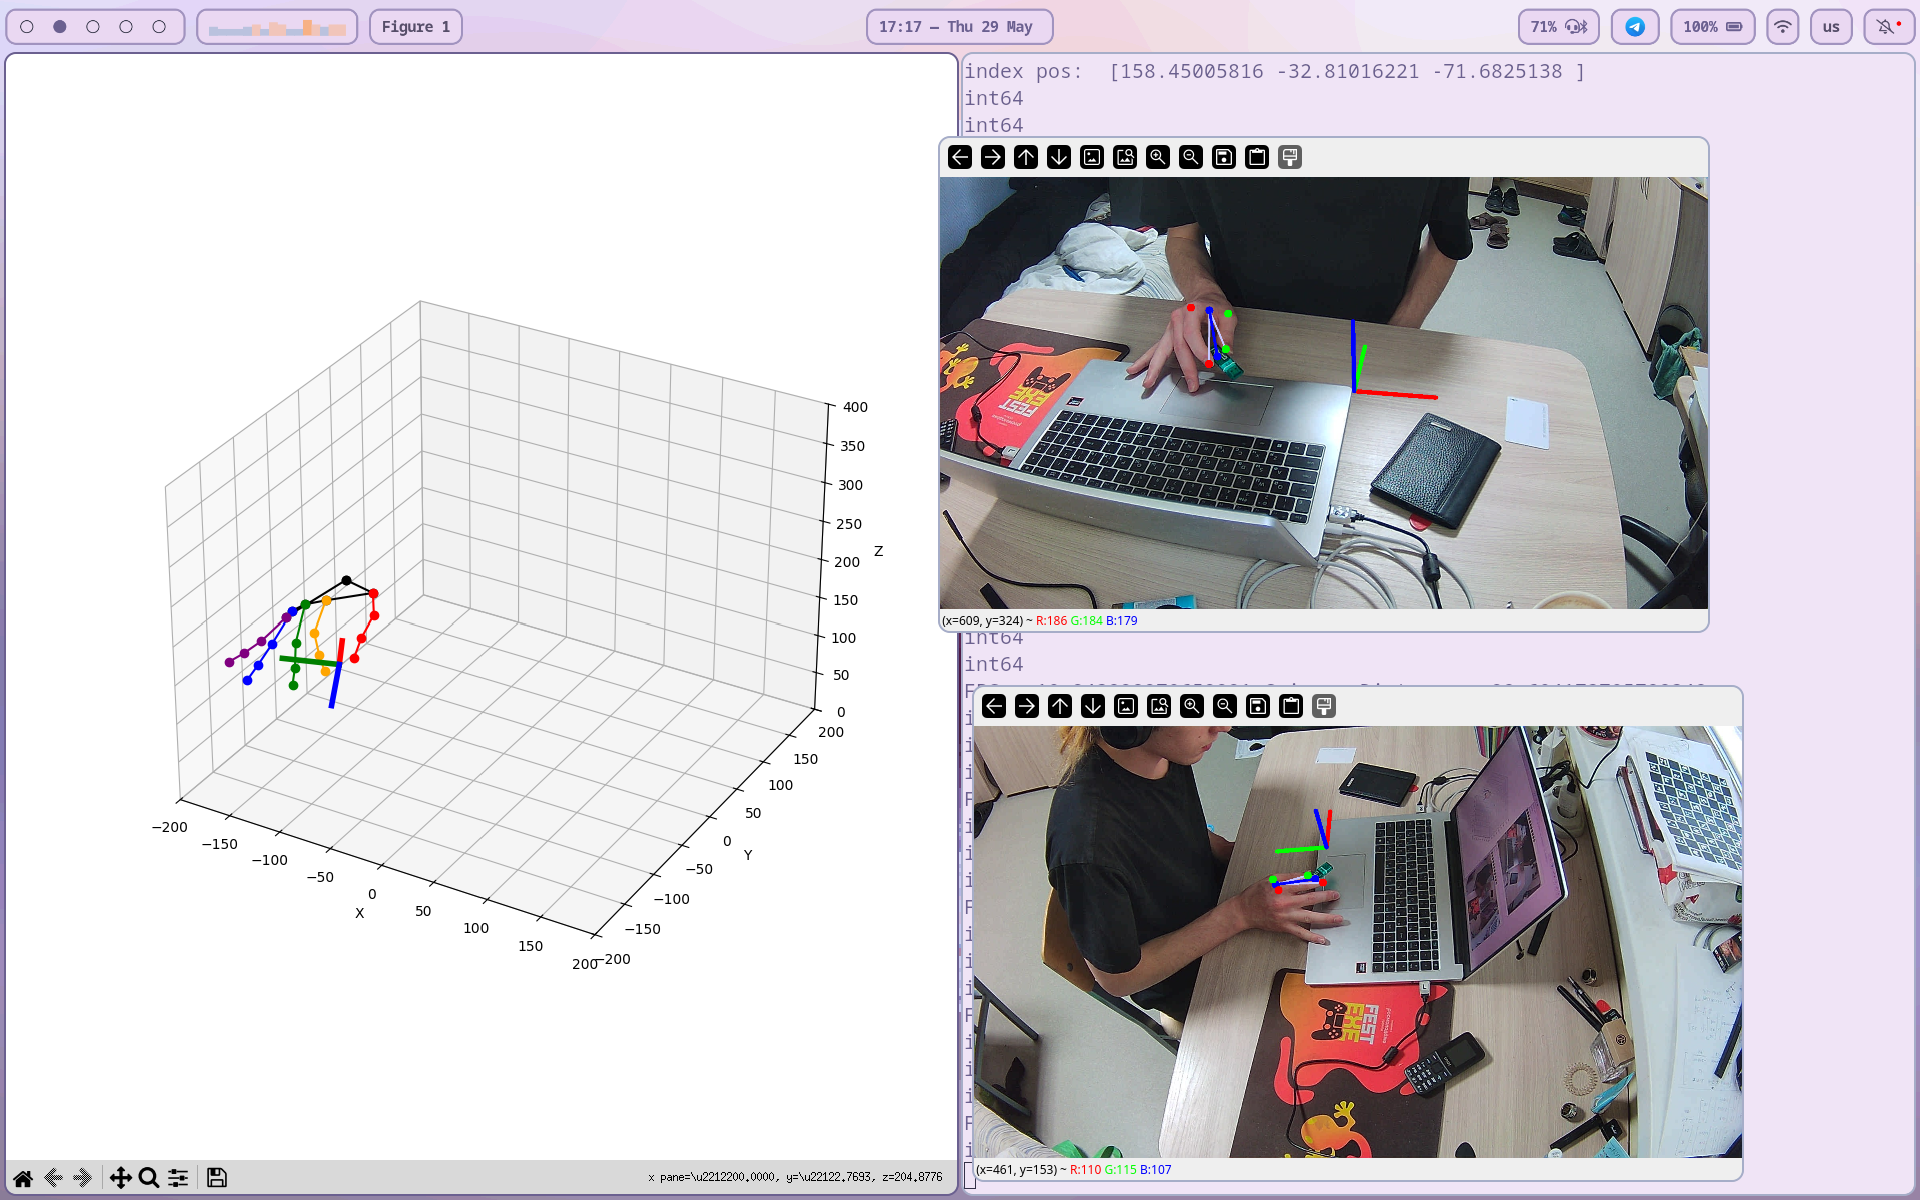
\includegraphics[width=0.7\textwidth]{images/gripper-conversion/gripper-conversion-3.png}\hfill
  \end{center}
  \caption{Отображение захвата в 3D и на кадрах с камеры}\label{fig:basic_gripper_work}
\end{figure}

Главным преимуществом данного метода является простота. Главным недостатком
является то, что этот метод крайне ограничен --- данный метод будет работать
лишь в ограниченном количестве ситуаций, где человек берет предмет таким
образом. Также, этот метод не очень надежен, во время тестирования, я заметил,
что даже если я беру предмет указательным и большим пальцами, предмет не всегда
взят подушечками пальцев, на которые расчитан этот метод.
\subsection{Интерфейс для приведения руки к захвату}
Для того, чтобы унифицировать методы приведения руки к захвату, сначала был
написан класс-интерфейс \texttt{GripperConverterInterface}, реализованный в
файле \texttt{gripper\_converter\_interface.py}.
При инициализации он принимает путь к конфигурации руки, где указаны индексы
сочленений в руке, открывает этот файл и сохраняет его в поле \texttt{named\_connections}.
\listingsection{
  ../gripper_conversion/gripper_converter_interface.py
}{INIT}

Также, я заранее указал на существование метода \texttt{get\_gripper\_state}.
Этот метод описывает, что передается на вход и что возвращается при
приведении руки к захвату.
На входе у этого метода один аргумент \texttt{points3d} --- массив из
координат каждой из ключевых точек руки.
Метод \texttt{get\_gripper\_state} возвращает список из трехмерных векторов
--- оси $X, Y$ и $Z$ инструментальной системы координат, трехмерный вектор
--- положение выходного звена и число с плавающей точкой --- расстояние, на
котрое нужно открыть захват.
\listingsection{
  ../gripper_conversion/gripper_converter_interface.py
}{STATE}

\subsection{Тестовый класс}
На ранних этапах разработки я написал более простой класс, который не
расчитывает степень раскрытия захвата, а ориентацию определяет по
указательному пальцу и вектору от костяшки указательного пальца к костяшке
среднего. Этот класс описан в файле \texttt{test\_gripper\_converter.py}.
При инициализации он сохраняет индексы необходимых шарниров чтобы потом
обращаться к ним. Это происходит в методе
\texttt{set\_orientation\_index\_z}, который вызывается на этапе
инициализации.
\listingsection{
  ../gripper_conversion/test_gripper_converter.py
}{INIT}
В методе \texttt{set\_orientation\_index\_z} сохраняются как поля класса индексы первого
сустава указательного пальца, то есть его костяшки, индекс конца
указательного пальца, а также индекс костяшки среднего пальца.
\listingsection{
  ../gripper_conversion/test_gripper_converter.py
}{SET_PARAMS}

Для получения состояния выходного звена ипользуется перегруженный метод
\texttt{get\_gripper\_state}. Сначала получаются координаты центра выходной
системы координат, который лежит в костяшке указательного пальца.
\listingsection{
  ../gripper_conversion/test_gripper_converter.py
}{CENTER}
Затем получются вектора осей $X$ и $Z$. Ось $X$ направлена от костяшки
указательного пальца к его концу, а ось $Z$, как раньше говорилось,
направлена от костяшки указательного к костяшке среднего.
\listingsection{
  ../gripper_conversion/test_gripper_converter.py
}{VECTORS}
Направление оси $Y$ расчитывается как векторное произведение осей $X$ и $Z$.
\listingsection{
  ../gripper_conversion/test_gripper_converter.py
}{YCALC}
Затем вектора $Y$ и $Z$ нормализуются.
\listingsection{
  ../gripper_conversion/test_gripper_converter.py
}{NORMALIZE}
В конце, чтобы ось $X$ точно была перпендикулярна двум другим, она
перерасчитывается как векторное произведение осей $Y$ и $Z$ и результат
возвращается.
\listingsection{
  ../gripper_conversion/test_gripper_converter.py
}{ORTHO}

 
\section{Заключение}
Целью этой работы было создание системы, котора позволить определить целевое
положение и ориентацию выходного звена манипулятора на основе данных с камер.
При этом нужно было реализовать отдельные модули для калибровки, распознавания
руки, расчета положения руки и приведения конфигурации руки человека к степени
захвата манипулятора.
  

В итоге эта система, была реализована. Запускалась на ноутбуке со следующими
характеристиками:
\begin{itemize}
  \item процессор --- AMD Ryzen 7 8845HS,
  \item ОЗУ --- 16 Гб,
  \item ОС --- ArchLinux 64-bit,
  \item версия ядра Linux --- 6.14.7.
\end{itemize}
В среднем, программа работает с частотой 14 Гц, чего будет достаточно для многих применений.
После проведения небольших измерений точности, было получено, что погрешность оценки
степени закрытия захвата лежит в диапазоне от 9 миллиметров до 16 миллиметров.
Одно из замечаний --- разброс значений ошибки мал для разных размеров. Можно
предположить, что для более больших объектов ошибка тоже будет иметь порядок
10-20 миллиметров. Замеры по точности проводилить следующим образом: при помощи
штангенциркуля измерялся габаритный размер какого-либо подручного предмета,
который человек может взять, я брал его в руку и запускал модификацию файла
\texttt{run\_hand\_positioning.py}, в которой считались и суммировались
квадраты значений ошибки. В конце исполнения, сумма делится на количетство
записанных ошибок и выводится на экран. Данные были собраны для нескольких
предметов с разными размерами. График зависимости погрешности от размера
взятого объекта представлен на рисунке \ref{fig:error-plot}. Данная точность не
подходит для точных действий, однако даже в текущем виде подобная система может
иметь свои применения, например, в сфере развлечений или для более грубых
действий. Систему, однако, можно улучшить несколькими способами, о которых речь
пойдет ниже.
\begin{figure}
  \begin{center}
    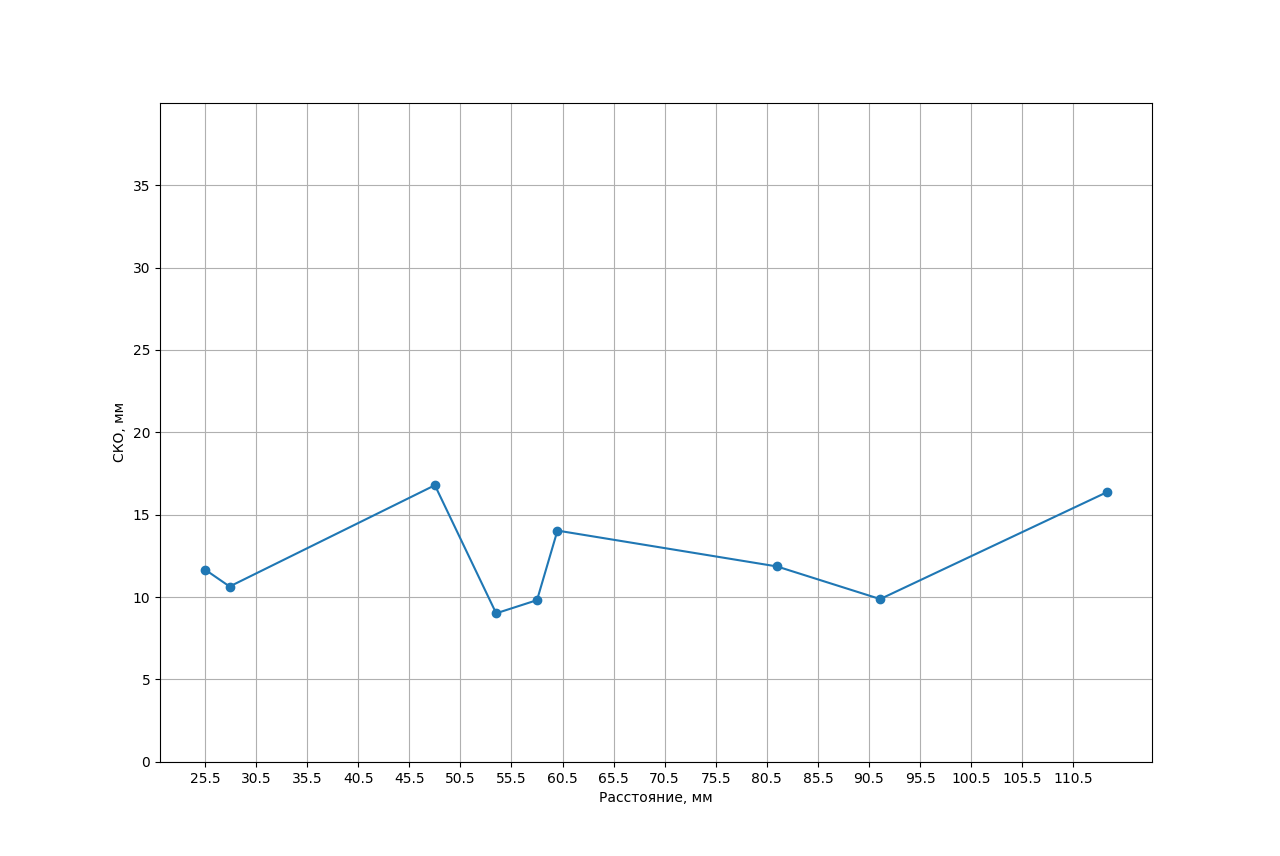
\includegraphics[width=0.95\textwidth]{images/error-plot.png}
  \end{center}
  \caption{Среднеквадратичное отклонение(СКО) в зависимости от размера взятого объекта}\label{fig:error-plot}
\end{figure}

Этап калибровки довольно сложно поддается алгоритмическим улучшениями, однако
улучшив оборудование можно сильно повысить качество калибровки как внутренних
параметров, так и положения. В этой работе проблема калибровки заключается в
том, что она проводилась при помощи доски ChArUco, распечатанной на листе
бумаги на домашнем принтере. Точность печати этого принтера неизвестна, а
обычная бумага легко деформируется. Комбинация этих факторов понижает качетво
полученных внутренних параметров. Также, улучшить точность системы можно при
помощи использования более качественных камер, которые будут иметь меньшие
коэффициенты искажения.

Распознавание рук работает далеко не идеально, предсказания модели сильно
варьируются даже когда рука не двигается, что понижает точность. С этим может
помочь применение фильтров для сглаживания предсказаний, а так же использование
более мощной модели, которой потребовались бы большие вычислительные мощности.
Также, с учетом наличия большого количества наборов данных, можно натренировать
свою модель на специфичном наборе данных, фокусирующимся только на взятии
предметов людьми. Однако более простым и необходимым улучшением все же является
фильтрация и сглаживание предсказаний.

Определение положения рук работает довольно хорошо для текущей реализации, в
которой не используются более сложные способы понижения шума. Однако точность
точно можно улучшить, использовав более продвинутые способы, описанные в
\cite{multiview_cv}. Также, на этом этапе можно сделать множество оптимизаций,
которые позволят программе работать на более высокой частоте. Главное, что
поможет с производительностью --- параллелизация исполнения программы. На
данный момент была лишь одна попытка сделать исполнение паралелльным и эта
попытка не используется в рабочей программе, а только в наброске.

Приведение к захвату манипулятора можно улучшить, реализовав любой из способов,
упомянутых в соответствующей секции. Чтобы повысить точность текущего метода
можно добавить дополнительное, более точное, определение точек контакта. На
данный момент, точки захвата определяются как центры пальцев, но человек,
очевидно, берет объекты не геометрическими центрами пальцев, а их краями. 
Также, большая универсальность необходима для более "серьезного" применния этой
системы.

На данный момент система может найти свое применение в сфере развлечений и
грубой телеоперации роботом, например, для перемещения больших объектов. Если
улучшить точность, то система может оказаться подходящей для телеоперации в
более требовательных к точности сферах, например, для записи датасетов. Другой
из вариантов --- работа в условиях, где человеку нельзя находиться,
но нужно манипулировать какими-либо предметами.

Полный исходный код проекта, включая код для LaTex загружен на платформу
github.com\cite{mycode-github}. Файлы pyproject.toml и hands\_env.yaml,
необходимые для правильной установки зависимостей находятся в приложениях, как
и весь используемый код.

\section{Приложения}
\subsection{intrinsics\_calibration.py}
\lstinputlisting[
    label=lst:intr_calib,
    caption={\texttt{intrinsics\_calibration.py}},
    language=python
    ]{../src/intrinsics_calibration.py}


\subsection{orientation\_calibration.py}
\lstinputlisting[
    label=lst:pos_calib,
    caption={\texttt{orientation\_calibration.py}},
    language=python
    ]{../src/orientation_calibration.py} 

\subsection{capture\_detector.py}
\lstinputlisting[
    label=lst:capture_detector,
    caption={capture\_detector.py},
    language=Python
    ]{../detection/capture_detector.py}
\subsection{Программа для запуска детекции}
\lstinputlisting[language=Python]{../src/run_detection.py}

\subsection{triangulator.py}
\lstinputlisting[language=Python]{../positioning/triangulator.py}

\subsection{run\_hand\_positioning.py}
\lstinputlisting[language=Python]{../src/run_hand_positioning.py}

\subsection{test\_gripper\_converter.py}
\lstinputlisting[language=Python]{../gripper_conversion/test_gripper_converter.py}

\subsection{visualizer\_3d.py}
\lstinputlisting[language=Python]{../utils/visualizer_3d.py}

\subsection{file\_utils.py}
\lstinputlisting[language=Python]{../utils/file_utils.py}

\printbibliography
% \bibliographystyle{plain}
% \bibliography{sources}
  
\end{document}
